\documentclass{beamer}
\usetheme[numbering=progressbar]{focus}
\definecolor{main}{RGB}{47, 161, 219}
\definecolor{textcolor}{RGB}{128, 128, 128}
\definecolor{background}{RGB}{240, 247, 255}

\usepackage[utf8]{inputenc}
\usepackage{tikz}
\usetikzlibrary{positioning,fit,calc,backgrounds}
\usetikzlibrary{shapes,arrows}

\usepackage{listings}
\usepackage[listings]{tcolorbox}
\tcbuselibrary{listings}
\lstdefinestyle{simple}{ %
    backgroundcolor=\color{gray!20},   % choose the background color; you must add \usepackage{color} or \usepackage{xcolor}; should come as last argument
    basicstyle=\ttfamily\tiny\color{black},        % the size of the fonts that are used for the code
    breakatwhitespace=false,         % sets if automatic breaks should only happen at whitespace
    breaklines=true,                 % sets automatic line breaking
    escapeinside={\%*}{*)},          % if you want to add LaTeX within your code
    extendedchars=true,              % lets you use non-ASCII characters; for 8-bits encodings only, does not work with UTF-8
    frame=single	                   % adds a frame around the code
    keepspaces=true,                 % keeps spaces in text, useful for keeping indentation of code (possibly needs columns=flexible)
    % language=json,                 % the language of the code
    %   keywordstyle=\bfseries,
    %   morekeywords={GET,POST,PUT,DELETE,... },           % if you want to add more keywords to the set
    numbers=none,                    % where to put the line-numbers; possible values are (none, left, right)
    numbersep=5pt,                   % how far the line-numbers are from the code
    numberstyle=\tiny\color{black}, % the style that is used for the line-numbers
    rulecolor=\color{black},         % if not set, the frame-color may be changed on line-breaks within not-black text (e.g. comments (green here))
    showspaces=false,                % show spaces everywhere adding particular underscores; it overrides 'showstringspaces'
    showstringspaces=false,          % underline spaces within strings only
    showtabs=false,                  % show tabs within strings adding particular underscores
    stepnumber=1,                    % the step between two line-numbers. If it's 1, each line will be numbered
    tabsize=2,	  
}
\lstset{style=simple}
\def\inline{\lstinline[basicstyle=\ttfamily\tiny\color{black}]}

\usepackage{xparse}
\usepackage{fontawesome}
\usepackage{xifthen}
\newcommand{\taggable}{\faicon{tags}\hspace*{0.3em}}
\newcommand{\distributable}{\faicon{eye-slash}\hspace*{0.3em}}
\newcommand{\synchronisable}{\faicon{exchange}\hspace*{0.3em}}

%
% Layout
%
\tikzstyle{mybox} = [
    draw=black,
    fill=white,
    very thick,
    rectangle, rounded corners,
    inner sep=10pt
]
\tikzstyle{boxtitle} = [
    % fill=black,
    % text=white,
    % fill=gray!30,
    % text=black,
    % font=\bfseries,
    % right=10pt
    draw=black,
    line width=1pt,
    text=white,
    fill=black!80,
    font=\bfseries,
    rectangle, rounded corners=2pt,
    inner sep=4pt,
    right=10pt
]
\tikzset{actionbox/.style={
    text=white,
    yshift=-1pt,xshift=-1pt,
    append after command={
    \pgfextra
            \draw[sharp corners, fill=black]% 
        (\tikzlastnode.west)% 
        [rounded corners=0pt] |- (\tikzlastnode.north)% 
        [rounded corners] -| (\tikzlastnode.east)% 
        [rounded corners=0pt] |- (\tikzlastnode.south)% 
        [rounded corners] -| (\tikzlastnode.west);
    \endpgfextra
    }
}}

% Creates a box with a label taking 1/3 of the available width
% arg1[optional] = icon
% arg2[optional] = purpose
% arg3[optional] = usecase
% arg4[optional] = actions
% arg5[optional] = description
% arg6 = title
% arg7 = content
\NewDocumentCommand{\cheatbox}{ O{} O{} O{} O{} O{} m m}{
    \begin{tikzpicture}
        \node [mybox] (box){%
            \begin{minipage}{0.95\linewidth}
            \ifthenelse{\isempty{#4}}{}{\vspace{1em}}
            \textit{#5}
            \vspace*{0.3em}
            \ifthenelse{\isempty{#2}}{}{ \par{\textbf{Purpose}: #2}}
            \ifthenelse{\isempty{#3}}{}{ \par{\textbf{Usecase}: #3\ifthenelse{\isempty{#7}}{}{\\}}}
            #7
            \end{minipage}
        };
        \node[boxtitle] at (box.north west) {#1 #6};
        \ifthenelse{\isempty{#4}}{}{
            \path node [actionbox, anchor=north east] at (box.north east) (actionLabel) {#4};
        }
    \end{tikzpicture}

    \vspace*{2pt}
}



\title{Mapping investigations and cases in MISP}
\subtitle{e.205}
\author{\small{CIRCL Computer Incident Response Center Luxembourg}}
\date{\today \hspace{3pt}- v0.7
}
\titlegraphic{
\includegraphics[scale=0.50]{misplogo.pdf}}
\institute{MISP Project \\ \url{https://www.misp-project.org/}}

\begin{document}
% DO NOT COMPILE THIS FILE DIRECTLY!
% This is included by the other .tex files.

\begin{frame}[t,plain]
\titlepage
\end{frame}

\begin{frame}
    \frametitle{Objectives of this module}
    \begin{itemize}
        \item Recap on MISP data model and distribution levels
        \item Data from cases to be structured and encoded:
        \begin{itemize}
            \item \textbf{Network indicators}: \texttt{ip}, \texttt{domain}, \texttt{url}, ...
            \item \textbf{Files and binaries}: non-malicious / malicious \texttt{payload}
            \item \textbf{Emails}: \texttt{content}, \texttt{header}, \texttt{attachment}, ...
            \item \textbf{Web}: \texttt{URL}, \texttt{cookies}, \texttt{x509}
            \item \textbf{Cryptographic materials}: public / private \texttt{key}, \texttt{certificate}
            \item \textbf{Infrastructure and devices}
            \item \textbf{Financial fraud}: \texttt{bank-account}, \texttt{phone-number}, \texttt{btc}
            \item \textbf{Person}: \texttt{name}, \texttt{online accounts}, \texttt{passport}, \texttt{visa}
            \item \textbf{Support tools}: \texttt{yara}, detection/remediation scripts
            \item \textbf{Vulnerabilities}: \texttt{cve}
            \item \textbf{External analysis}: Reports, blogpost, ransome notes
        \end{itemize}
        \item Relationships and timeliness
        \item Enrichments via module and correlation
        \item Preparing data for sharing with other LE partners, CSIRT, SOC
    \end{itemize}
\end{frame}

\section{MISP Data model and distribution levels}
\begin{frame}
    \frametitle{MISP Event}

    \cheatbox[\faicon{envelope}]
        [Group datapoints and context together. Acting as an envelop, it allows setting distribution and sharing rules for itself and its children.]
        [Encode incidents/events/reports/…]
        [\taggable \distributable \synchronisable]
        [Encapsulations for contextually linked information.]
        {Event}
        {
            $\blacktriangleright$ events can contain other elements such as attributes, objects and eventreports.\\
            $\blacktriangleright$ The distribution level and any context added on an event (such as taxonomies) are propagated to its underlying data.
        }
\end{frame}

\begin{frame}
    \frametitle{MISP Attribute}

    \cheatbox[\faicon{cube}]
        [Individual data point. Can be an indicator or supporting data.]
        [Domain, IP, link, sha1, attachment, …]
        [\taggable \distributable \synchronisable]
        [Basic building block to share information.]
        {Attribute}
        {
            $\blacktriangleright$ attributes cannot be duplicated inside the same event and can have sightings.\\
            $\blacktriangleright$ The difference between an indicator or supporting data is usualy indicated by the state of the attribute's \texttt{to\_ids} flag.
        }
\end{frame}

\begin{frame}
    \frametitle{MISP Object}

    \cheatbox[\faicon{cubes}]
        [Groups attributes that are intrinsically linked together.]
        [File, person, credit-card, x509, device, \dots]
        [\distributable \synchronisable]
        [Advanced building block providing attribute compositions via templates.]
        {MISP Object}
        {
            $\blacktriangleright$ objects have their attribute compositions described in their respective template. They are instanciated with attributes and can reference other attributes or objects.\\
            $\blacktriangleright$ MISP is not required to know the template to save and display the object. However, \textit{edits} will not be possible as the template to validate against is unknown.
        }

\end{frame}

\begin{frame}
    \frametitle{MISP Relationships (aka object reference)}

    \cheatbox[$\nearrow$]
        [Allows to create relationships between entities, thus creating a graph where they are the edges and entities are the nodes.]
        [Represent behaviours, similarities, affiliation, \dots]
        [\synchronisable]
        [Relationships between individual building blocks.]
        {Object Reference}
        {
            $\blacktriangleright$ references can have a textual relationship which can come from MISP or be set freely.
        }
\end{frame}

\begin{frame}
    \frametitle{MISP Event report}

    \cheatbox[\faicon{file-text}]
        [Supporting data point to describe events or processes.]
        [Encode reports, provide more information about the event, \dots]
        [\distributable \synchronisable]
        [Advanced building block containing formated text.]
        {Event Report}
        {
            $\blacktriangleright$ Event reports are markdown-aware and include a special syntax to reference data points or context.
        }
\end{frame}


\begin{frame}
    \frametitle{General rule of thumb}

    Which structure should be used when encoding data?
    \begin{itemize}
        \item \textbf{Attribute} vs \textbf{Object}
        \begin{itemize}
            \item If the value is contextually linked to another element or is a subpart of a higher concept, an \textbf{object} should be used
            \item If the value is part of a large list of atomic data, an \textbf{attribute} should be used
        \end{itemize}
        \item \textbf{\texttt{Annotation} Object} vs \textbf{Event Report}
        \begin{itemize}
            \item If it is possible to encode the text (raw text or markdown), an \textbf{event report} is prefered
            \item If the text is written in a specific format (e.g pdf, docx), an \textbf{\texttt{annotation} object} should be used
        \end{itemize}
    \end{itemize}
\end{frame}

\section{Case study 1: Scam call}
\begin{frame}
    \frametitle{Case study 1: Scam call}
    % event uuid: 53d2f469-9f7f-4e40-8dc1-a721f1b223fb
    \begin{itemize}
        \item[] \textbf{Case}: A victim was asked to transfer money to a novice scammer
        \item[] \textbf{Chronology - 2022-03-24}
        \begin{itemize}
            \item[] \textbf{\small 11:42:43 UTC+0}: Scammer called the victim pretending to be a microsoft employee
            \item[] \textbf{\small 11:47:27 UTC+0}: Scammer convinced the victim to be helped via remote desktop assistance
            \item[] \textbf{\small 12:06:32 UTC+0}: Scammer downloaded the binary on the victim's computer
            \item[] \textbf{\small 12:08:18 UTC+0}: Scammer installed the binary on the victim's computer
            \item[] \textbf{\small 12:17:51 UTC+0}: Scammer asked the victim to transfer money on a bank account for the help he provided
            \item[] \textbf{\small 12:25:04 UTC+0}: Victim executed the money transfer
            \item[] \textbf{\small 2022-03-25 08:39:21 UTC+0}: Victim contacted police
        \end{itemize}
    \end{itemize}
\end{frame}

\begin{frame}
    \frametitle{Case study 1: Scam call}
    \begin{itemize}
        \item[] \textbf{Collected evidences}
        \begin{itemize}
            \item RDP Log file
            \item Installed binary
            \item Victim's browser history
            \item Bank account statement
            \item Victim's phone call log
        \end{itemize}
    \end{itemize}
    \begin{itemize}
        \item[] \textbf{Data extracted from evidences}
        \begin{itemize}
            \item Scammer's \textbf{ip address}
            \item Potentially \textbf{malicious binary}
            \item \textbf{URL} (and \textbf{domain}) from which the binary was downloaded
            \item Scammer's \textbf{bank account} and \textbf{phone number}
            \item Scammer's full name and nationality
        \end{itemize}
    \end{itemize}
\end{frame}

\begin{frame}
    \frametitle{Case study 1: Scam call}
    \begin{itemize}
        \item[] \textbf{Extracted values}
        \begin{itemize}
            \item \texttt{\color{black} 194.78.89.250}
            \begin{itemize}
                \item ip-address from log file
            \end{itemize}
            \item \texttt{\color{black} bin.exe}
            \begin{itemize}
                \item downloaded binary
            \end{itemize}
            \item \texttt{\color{black} https://zdgyot.ugic0k.ru/assets/bin.exe}
            \begin{itemize}
                \item download URL
            \end{itemize}
            \item \texttt{\color{black} GB 29 NWBK 601613 31926819 }
            \begin{itemize}
                \item IBAN number
                \item Swift: \texttt{\color{black} NWBK}, Account number: \texttt{\color{black} 31926819}, Currency: \texttt{\color{black} GBP}
            \end{itemize}
            \item \texttt{\color{black} +12243359185}
            \begin{itemize}
                \item phone number
            \end{itemize}
            \item \texttt{\color{black} Wallace Breen} is from \texttt{\color{black} GB}
            \begin{itemize}
                \item name and nationality
            \end{itemize}
        \end{itemize}
    \end{itemize}

    \note[item]{We are dealing with fake values}
\end{frame}

\begin{frame}
    \frametitle{Case study 1: Scam call}
    \begin{itemize}
        \item[] \textbf{Tasks}
        \begin{itemize}
            \item Create an new \textit{event} to be shared with \textbf{all}
            \item Encode \texttt{binary} to be shared with \textbf{CSIRT}
            \item Encode \texttt{ip address} to be shared with both \textbf{ISP} and \textbf{CSIRT}
            \item Encode \texttt{domain} and \texttt{url} to be shared with both \textbf{ISP} and \textbf{CSIRT}
            \item Encode \texttt{bank account} to be shared with \textbf{Financial sector}
            \item Encode \texttt{phone number} to be shared with \textbf{Telecomunication sector}
            \item Encode \texttt{full name} and \texttt{nationality} to be shared with \textbf{LEA only}
            \item Add relationships to recreate the events
            \item Add time component to recreate the chronology
            \item Perform enrichments on the binary, and other attribute
            \item Add contextualization
            \item Create a small write-up as an \textit{event report}
            \item Review the distribution level and publish
        \end{itemize}
    \end{itemize}
\end{frame}

\begin{frame}
    \frametitle{Case study 1: Scam call}
    \begin{itemize}
        \item Creating the \textit{event} in MISP
    \end{itemize}
    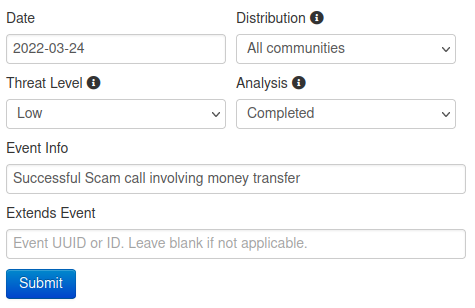
\includegraphics[width=1.0\linewidth]{pictures/case1/event.png}
\end{frame}

\begin{frame}
    \frametitle{Case study 1: Scam call}
    \begin{itemize}
        \item Adding the binary as attachment
        \item Pick the \texttt{Payload Delivery} category
        \item Check \textit{Is a malware sample}
    \end{itemize}
    \begin{center}
        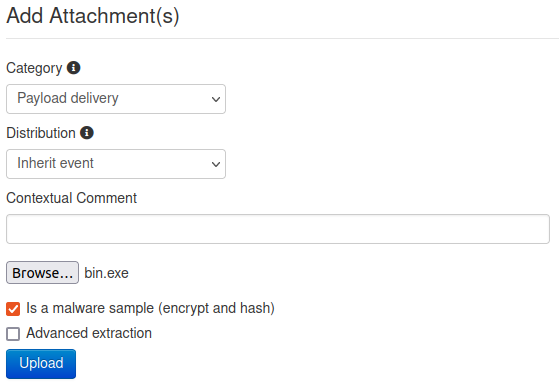
\includegraphics[width=0.80\linewidth]{pictures/case1/attribute-bin.png}
    \end{center}
\end{frame}

\begin{frame}
    \frametitle{Case study 1: Scam call}
    \begin{itemize}
        \item Encode the IP address of the scammer with an \textit{attribute}
        \item Pick the \texttt{Payload Installation} category and \texttt{ip-src}  \texttt{type}
        \item Check the \texttt{For Intrusion Detection System}
        \item Add a contextual comment such as
        \begin{itemize}
            \item \texttt{IP address of the scammer collected from the RDP log file}
        \end{itemize}
    \end{itemize}
    \begin{center}
        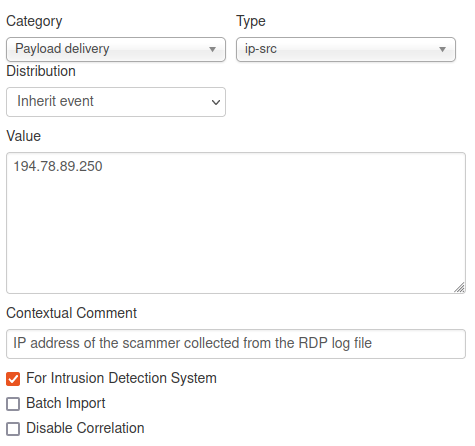
\includegraphics[width=0.63\linewidth]{pictures/case1/attribute-ip.png}
    \end{center}
\end{frame}

\begin{frame}
    \frametitle{Case study 1: Scam call}
    \begin{itemize}
        \item Encode the domain and the URL from which the binary was downloaded
        \item As these two attributes are contextually linked between each others, we should use an \texttt{URL} \textit{object}
        \item Add a contextual comment such as
        \begin{itemize}
            \item \texttt{URL used by the scammer to download the binary}
        \end{itemize}
        \item Include at least: \texttt{url}, \texttt{domain} and \texttt{ressource\_path}
    \end{itemize}
\end{frame}

\begin{frame}
    \frametitle{Case study 1: Scam call}
    \begin{center}
        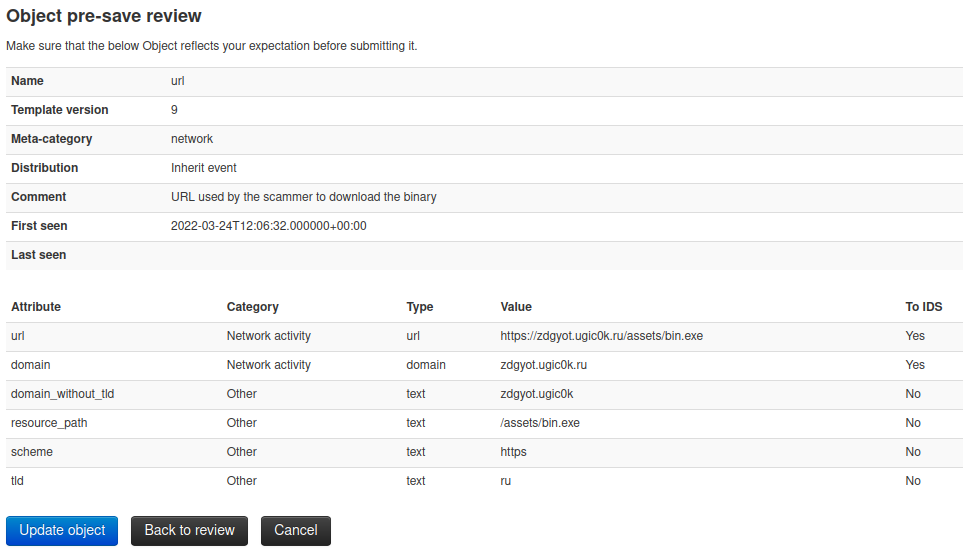
\includegraphics[width=1.0\linewidth]{pictures/case1/object-url.png}
    \end{center}
\end{frame}

\begin{frame}
    \frametitle{Case study 1: Scam call}
    \begin{itemize}
        \item Encode the bank account
        \item As these 4 attributes are contextually linked between each others, we should use an \texttt{bank-account} \textit{object}
        \item Add a contextual comment such as
        \begin{itemize}
            \item \texttt{Bank account that received the money. Supposed to belong to the scammer}
        \end{itemize}
        \item Include at least: \texttt{iban}, \texttt{swift}, \texttt{account} and \texttt{currency\_code}
    \end{itemize}
\end{frame}

\begin{frame}
    \frametitle{Case study 1: Scam call}
    \begin{center}
        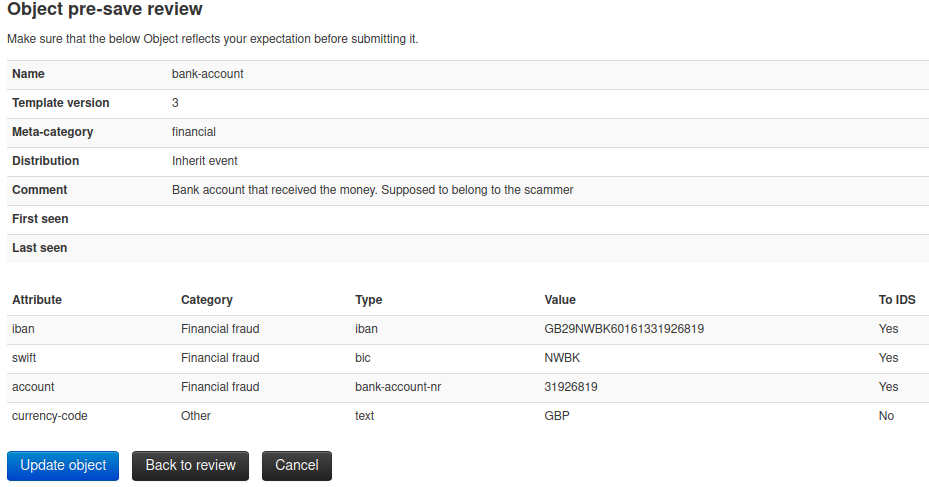
\includegraphics[width=1.0\linewidth]{pictures/case1/object-bankaccount.png}
    \end{center}
\end{frame}

\begin{frame}
    \frametitle{Case study 1: Scam call}
    \begin{itemize}
        \item Encode the phone number
        \item Pick the \texttt{Financial Fraud} category and \texttt{phone-number} \texttt{type}
        \item Add a contextual comment such as
        \begin{itemize}
            \item \texttt{Phone number used by the scammer to call the victim}
        \end{itemize}
        \item Check \textit{For Intrusion Detection System}
    \end{itemize}
    \begin{center}
        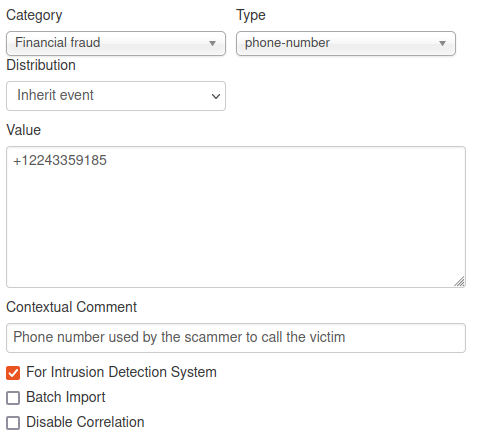
\includegraphics[width=0.70\linewidth]{pictures/case1/attribute-phone.png}
    \end{center}
\end{frame}

\begin{frame}
    \frametitle{Case study 1: Scam call}
    \begin{itemize}
        \item Encode the full name and nationality
        \item As these attributes are contextually linked between each others, we should use a \texttt{person} \textit{object}
        \item Add a contextual comment such as
        \begin{itemize}
            \item \texttt{Name of the scammer given to the victim}
        \end{itemize}
        \item Include at least: \texttt{full-name}, \texttt{nationality} and \texttt{role}
    \end{itemize}
\end{frame}

\begin{frame}
    \frametitle{Case study 1: Scam call}
    \begin{center}
        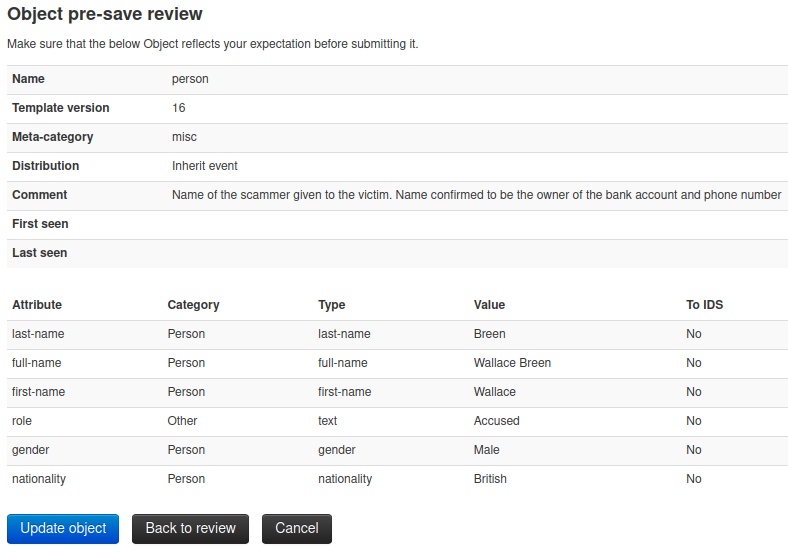
\includegraphics[width=1.0\linewidth]{pictures/case1/object-person.png}
    \end{center}
\end{frame}

\begin{frame}
    \frametitle{Case study 1: Scam call}
    Add (at least) these relationships to recreate the story

    \begin{center}
        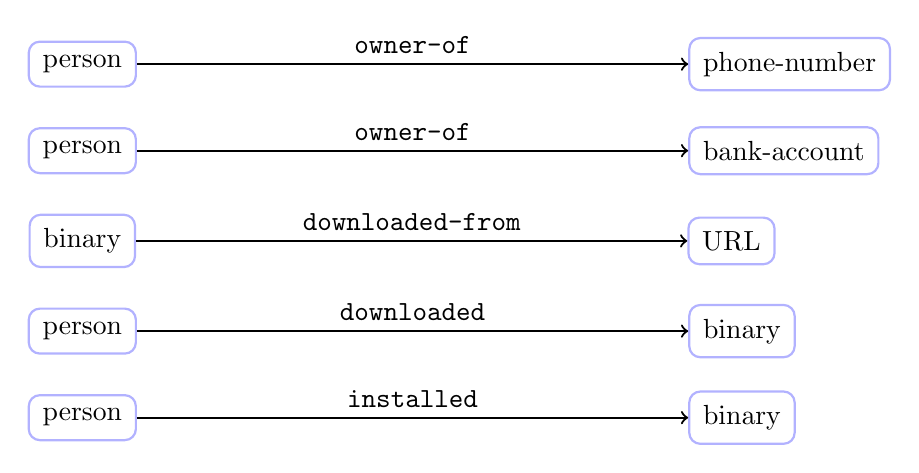
\begin{tikzpicture}[
            entity/.style={rectangle, draw=black, scale=1.0},
            simplebox/.style={
                rectangle, rounded corners, thick,
                draw=blue!30,
                minimum width=10pt,
                minimum height=10pt,
                inner sep=5pt, inner ysep=5pt
            },
        ]

            \node [simplebox] (person1)                     {person};
            \node [simplebox] (phone-number) [ right= 7cm of person1 ] {phone-number};
            \draw[->,thick] (person1) -- (phone-number) node [above,midway] {\texttt{owner-of}};

            \node [simplebox] (person2) [ below= 0.5cm of person1]       {person};
            \node [simplebox] (bank-account) [ right= 7cm of person2 ] {bank-account};
            \draw[->,thick] (person2) -- (bank-account) node [above,midway] {\texttt{owner-of}};

            \node [simplebox] (binary) [ below= 0.5cm of person2 ] {binary};
            \node [simplebox] (url)    [ right= 7cm of binary ] {URL};
            \draw[->,thick] (binary) -- (url) node [above,midway] {\texttt{downloaded-from}};

            \node [simplebox] (person3) [ below= 0.5cm of binary ] {person};
            \node [simplebox] (binary)  [ right= 7cm of person3 ] {binary};
            \draw[->,thick] (person3) -- (binary) node [above,midway] {\texttt{downloaded}};

            \node [simplebox] (person4) [ below= 0.5cm of person3 ] {person};
            \node [simplebox] (binary)  [ right= 7cm of person4 ]  {binary};
            \draw[->,thick] (person4) -- (binary) node [above,midway] {\texttt{installed}};

        \end{tikzpicture}
    \end{center}
\end{frame}

\begin{frame}
    \frametitle{Case study 1: Scam call}
    Add relationships to recreate the story
    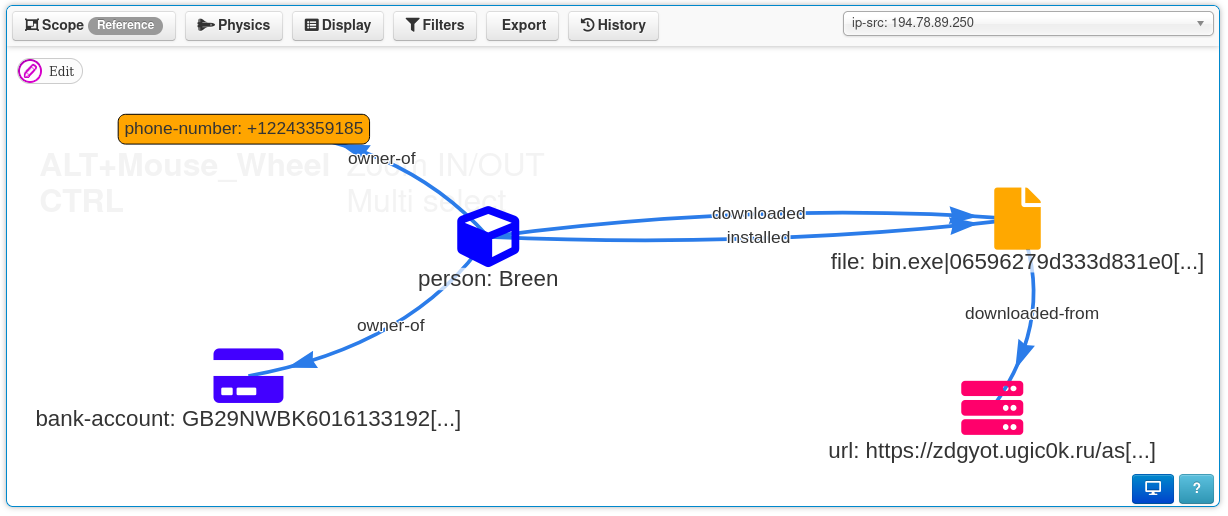
\includegraphics[width=1.0\linewidth]{pictures/case1/event-graph.png}
\end{frame}

\begin{frame}
    \frametitle{Case study 1: Scam call}
    Add time component to recreate the chronology
    \begin{itemize}
        \item Main focus is the Cyber Threat Intelligence (CTI) aspect
    \end{itemize}
    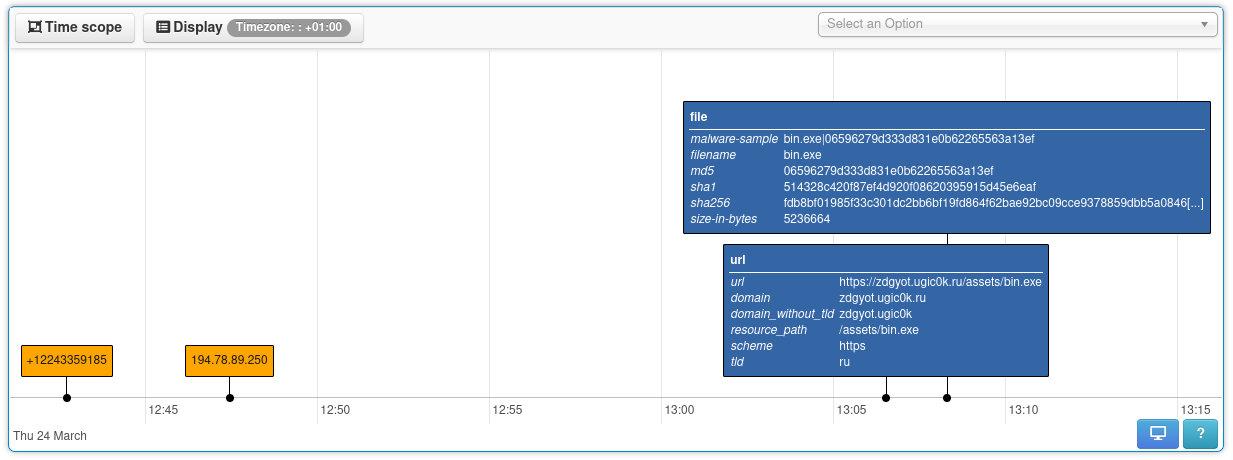
\includegraphics[width=1.0\linewidth]{pictures/case1/timeline.png}
\end{frame}

\begin{frame}
    \frametitle{Case study 1: Scam call}
    Perform enrichments
    \begin{itemize}
        \item Scammer IP address to get its location
        \item Binary to check if it's an existing (and malicious) application
    \end{itemize}
    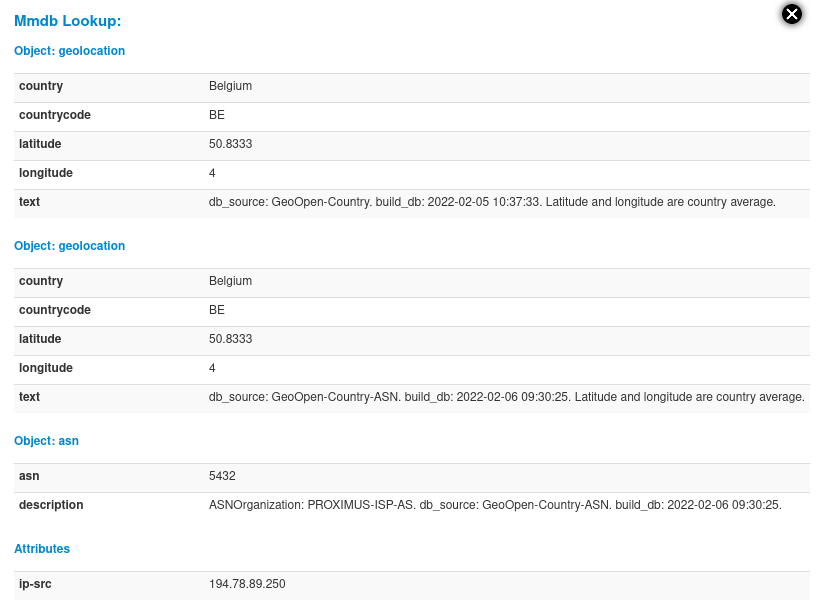
\includegraphics[width=1.0\linewidth]{pictures/case1/enrichment.png}
\end{frame}

\begin{frame}
    \frametitle{Case study 1: Scam call}
    \begin{itemize}
        \item Contextualizing the data: Taxonomies
        \begin{itemize}
            \item Note: Different country / sectors might use different nomemclature
        \end{itemize}
        \item Suggestions for tagging with taxonomies:
        \begin{itemize}
            \item \texttt{circl:incident-classification="scam"}
            \item \texttt{\tiny social-engineering-attack-vectors:non-technical="technical-expert"}
            \item \texttt{\tiny social-engineering-attack-vectors:technical="vishing"}
            \item \texttt{veris:action:hacking:vector="Desktop sharing"}
            \item \texttt{veris:action:malware:vector="Direct install"}
            \item \texttt{veris:action:social:variety="Scam"}
            \item \texttt{veris:action:social:vector="Phone"}
            \item \texttt{veris:actor:external:motive="Financial"}
            \item \texttt{veris:impact:loss:rating="Minor"}
            \item \texttt{veris:impact:loss:variety="Asset and fraud"}
            \item \texttt{workflow:state="complete"}
            \item \texttt{tlp:green}
        \end{itemize}
    \end{itemize}
\end{frame}

\begin{frame}
    \frametitle{Case study 1: Scam call}
    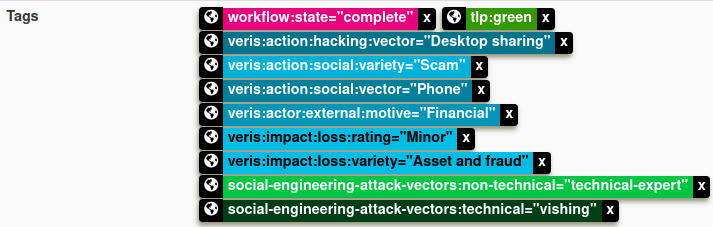
\includegraphics[width=1.0\linewidth]{pictures/case1/event-tags.png}
\end{frame}

\begin{frame}
    \frametitle{Case study 1: Scam call}
    \begin{itemize}
        \item Contextualizing the data: Galaxy Clusters
        \begin{itemize}
            \item Note: Different country / sectors might use different nomemclature
        \end{itemize}
        \item Suggestions for tagging with Galaxies:
        \begin{itemize}
            \item MITRE Attack Pattern
        \end{itemize}
    \end{itemize}
    \vspace{1cm}
    
\includegraphics[width=1.0\linewidth]{pictures/case1/event-clusters.png}
\end{frame}

\begin{frame}
    \frametitle{Case study 2: Ransomware}
    Preventive measures
    \begin{center}
        TODO: Include PM
        % \includegraphics[width=0.80\linewidth]{pictures/case2/event-clusters2.png}
    \end{center}
\end{frame}

\begin{frame}
    \frametitle{Case study 1: Scam call}
    Create a small write-up as an \textit{event report}
    \begin{itemize}
        \item Create the \textit{event report} with a concise name
        \item Example: Executive summary of the case
        \begin{itemize}
            \item Leave its content empty as it can be edited with more ease in the editor afterward
        \end{itemize}
        \item Write a summary with
        \begin{itemize}
            \item Quick chronology
            \item Written explanation of the steps tooks by the scammer
            \item Reference to existing \textit{attributes} or \textit{objects} whenever possible
            \begin{itemize}
                \item The special syntax is: \texttt{@[scope]\{uuid\}}
            \end{itemize}
        \end{itemize}
    \end{itemize}
\end{frame}

\begin{frame}
    \frametitle{Case study 1: Scam call}
    Create a small write-up as an \textit{event report}
    \begin{center}
        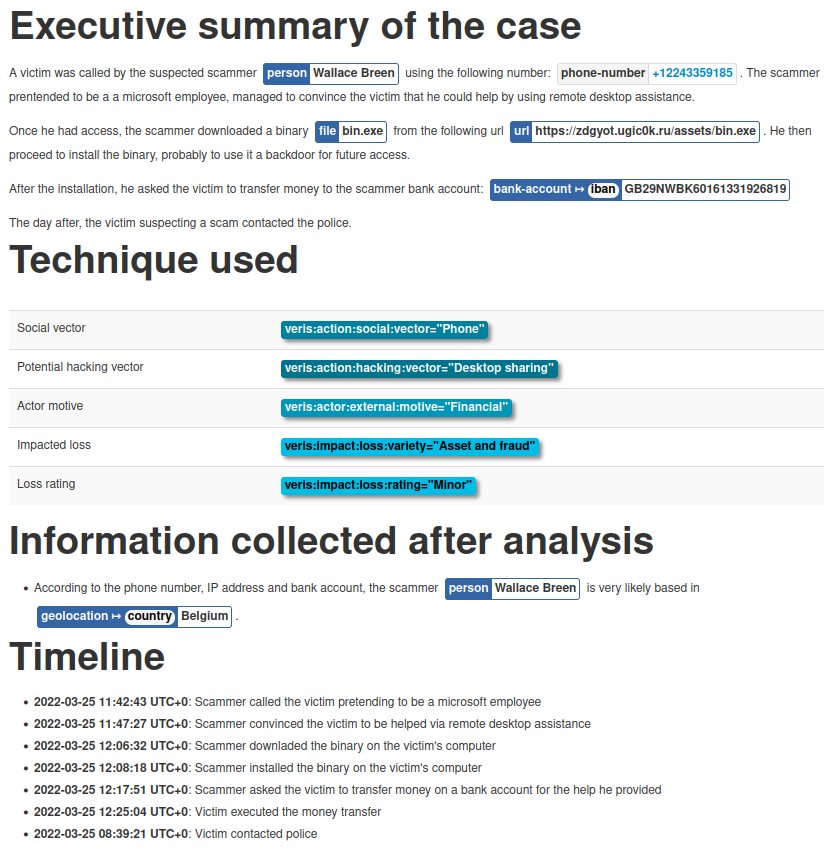
\includegraphics[width=0.65\linewidth]{pictures/case1/event-report.png}
    \end{center}
\end{frame}

\begin{frame}
    \frametitles{Case study 1: Scam call}{Review the distribution level and publish}
    In our case, we consider the following MISP network topology
    \begin{itemize}
        \item The current instance is owned and managed by a LEA
        \item The current instance is connected to a central MISP instance acting as a "Hub"
        \item The "Hub" is connected to various other MISP instances such as other LEAs, CSIRTs, Financial and telecom institutions
    \end{itemize}

    \begin{center}
        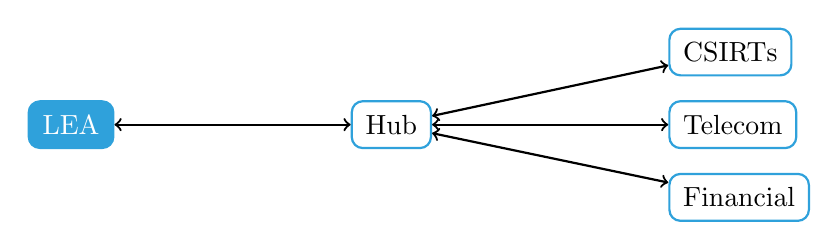
\begin{tikzpicture}[
            entity/.style={rectangle, draw=black, scale=0.7},
            simplebox/.style={
                rectangle, rounded corners, thick,
                draw=main,
                minimum width=10pt,
                minimum height=10pt,
                inner sep=5pt, inner ysep=5pt
            },
        ]
            \node [simplebox] (hub)                     {Hub};
            \node [simplebox,fill=main] (lea) [ left= 3cm of hub ] {\textcolor{white}{LEA}};
            \node [simplebox] (csirts) [ above right = 0.3cm and 3cm of hub ] {CSIRTs};
            \node [simplebox] (telecom) [ right= 3cm of hub ] {Telecom};
            \node [simplebox] (financial) [ below right= 0.3cm and 3cm of hub ] {Financial};

            \draw[<->,thick] (lea) -- (hub) node [above,midway] {};
            \draw[<->,thick] (csirts) -- (hub) node [above,midway] {};
            \draw[<->,thick] (telecom) -- (hub) node [above,midway] {};
            \draw[<->,thick] (financial) -- (hub) node [above,midway] {};

        \end{tikzpicture}
    \end{center}
\end{frame}

\begin{frame}
    \frametitle{Case study 1: Scam call}
    Review the distribution level and publish
    \begin{itemize}
        \item \texttt{binary file}: \textbf{All communities}
        \item \texttt{person}: \textbf{LEA Sharing group}
        \item \texttt{geolocation}: \textbf{LEA Sharing group}
        \item \texttt{ip}: \textbf{LEA Sharing group}
        \begin{itemize}
            \item The IP might be reassigned
        \end{itemize}
        \item \texttt{phone}
        \begin{itemize}
            \item If part of a telco sharing group \textbf{Telco Sharing group}
            \item \textbf{Connected communities} otherwise
        \end{itemize}
        \item \texttt{bank account}
        \begin{itemize}
            \item If part of a financial sharing group \textbf{Financial Sharing group}
            \item \textbf{Connected communities} otherwise
        \end{itemize}
    \end{itemize}
    \begin{center}
        \textbf{$\rightarrow$ Publish the event!}
    \end{center}
\end{frame}


%
%
% CASE 2
%
%

\section{Case study 2: Ransomware}
% cc8d930b-aa5f-40b8-a30e-dc86bfd83003 
\begin{frame}
    \frametitle{Case study 2: Ransomware}
    \begin{itemize}
        \item[] \textbf{Case}: Ransomware infection via e-mail
        \item[] \textbf{Chronology - 2022-03-24}
        \begin{itemize}
            \item[] \textbf{\small 11:42:43 UTC+0}: Email containing the ransomware from supposedly Andrew Ryan
            \item[] \textbf{\small 11:47:27 UTC+0}: Email was read and its attachment opened and executed
            \item[] \textbf{\small 11:47:28 UTC+0}: Malware add persistence
            \item[] \textbf{\small 12:08:18 UTC+0}: Malware successfully contacted the C2 to get the PK 
            \item[] \textbf{\small 12:08:19 UTC+0}: Malware saved the PK in the registry
            \item[] \textbf{\small 12:25:04 UTC+0}: Malware began the encryption process
            \item[] \textbf{\small 2022-03-25 08:39:21 UTC+0}: Victim contacted the police
        \end{itemize}
    \end{itemize}
\end{frame}

\begin{frame}
    \frametitle{Case study 2: Ransomware}
    Splash message from the Ransomware
    \begin{center}
        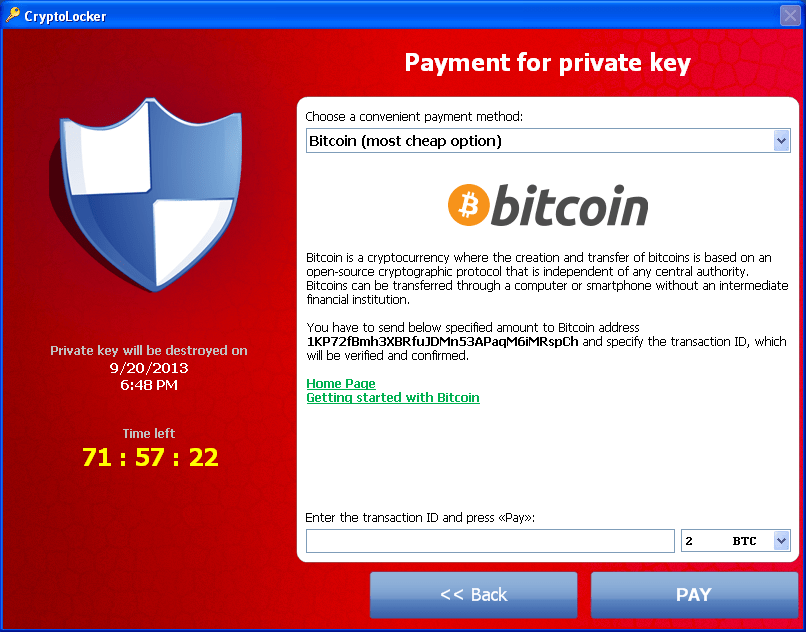
\includegraphics[width=0.8\linewidth]{./pictures/case2/ransom-btc.png}
    \end{center}
\end{frame}

\begin{frame}
    \frametitle{Case study 2: Ransomware}
    \begin{itemize}
        \item[] \textbf{Collected evidences}
        \begin{itemize}
            \item E-mail received by the victim
            \item E-mail attachment of the ransomware as an .exe payload
            \item Windows registry
            \item Ransomware's public key (PK)
            \item Captured network traffic
            \item Message displayed by the ransomware
        \end{itemize}
    \end{itemize}
    \begin{itemize}
        \item[] \textbf{Data extracted from evidences}
        \begin{itemize}
            \item Original \textbf{e-mail}
            \item The actual ransomware \textbf{binary}
            \item \textbf{Registry Keys} for persistence and configuration
            \item \textbf{Public Key} used for encryption
            \item C\&C server \textbf{ip address} used to generate the Private Key (SK)
            \item The \textbf{bitcoin address} on which the ransom should be paid
            \item The \textbf{person}, impersonated or fake that sent the email
        \end{itemize}
    \end{itemize}
\end{frame}

\begin{frame}[fragile]
    \frametitle{Case study 2: Ransomware}
\begin{lstlisting}[basicstyle=\tiny\color{black}]
Subject: 4829-2375
From: "Andrew_Ryan" <Andrew_Ryan@rindustries.rp>

Please see the attached Iolta report for 4829-2375.

We received a check request in the amount of $19,637.28 for the above referenced file. However, the attached report refects a $0 balance. At your earliest convenience, please advise how this request is to be funded.

Thanks.

Andrew_Ryan *
Accounts Payable

Ryan Industries
42, Central Control Hephaestus - Rapture
www.rindustries.rp

*Not licensed to practise law.

This communication contains information that is intended only for the recipient named and may be privileged, confidential, subject to the attorney-client privilege, and/or exempt from disclosure under applicable law. If you are not the intended recipient or agent responsible for delivering this communication to the intended recipient, you are hereby notified that you have received this communication in error, and that any review, disclosure, dissemination, distribution, use, or copying of this communication is STRICTLY PROHIBITED. If you have received this communication in error, please notify us immediately by telephone at 1-800-766-7751 or 1-972-643-6600 and destroy the material in its entirety, whether in electronic or hard copy format.
\end{lstlisting}

    \note[item]{We are dealing with fake values}
\end{frame}

\begin{frame}[fragile]
    \frametitle{Case study 2: Ransomware}
    \begin{itemize}
        \item[] \textbf{Extracted values}
        \begin{itemize}
            \item \texttt{e-mail} from previous slide
            \item \texttt{\color{black} cryptolocker.exe}
            \begin{itemize}
                \item Ransomware attached to the mail
            \end{itemize}
            \item \texttt{\color{black} 81.177.170.166}
            \begin{itemize}
                \item ip-address of a C2 server used to generate the SK
            \end{itemize}
            \item \lstinline|HKCU\SOFTWARE\Microsoft\Windows\CurrentVersion\Run "CryptoLocker"|
            \begin{itemize}
                \item The registry key used for persistence
            \end{itemize}
            \item \lstinline|HKCU\SOFTWARE\CryptoLocker VersionInfo|
            \begin{itemize}
                \item The registry key containing configuration data
            \end{itemize}
            \item \lstinline|HKCU\SOFTWARE\CryptoLocker PublicKey|
            \begin{itemize}
                \item The registry key containing the RSA public key received from the C2 server
            \end{itemize}
            \item \texttt{\color{black} 0x819C33AE}
            \begin{itemize}
                \item XOR key used to encode the configuration data
            \end{itemize}
        \end{itemize}
    \end{itemize}

    \note[item]{We are dealing with fake values}
\end{frame}

\begin{frame}[fragile]
    \frametitle{Case study 2: Ransomware}
    \begin{itemize}
        \item \begin{lstlisting}
-----BEGIN PUBLIC KEY-----
MIGfMA0GCSqGSIb3DQEBAQUAA4GNADCBiQKBgQDaogllvHPytDAdUWZPk9aWXJ5G
Lk9F+HzDaj5qGXou8XmISwChbia/NC84QmBHTiyg4B1tqVjqk5X6yh6pcZuVw+GX
0CrH5O5o2Q0XVYzYYsEZQB36VHxwm7xTx21yOy2rSOQyOupQ6e7HMGtu7p7+RlWO
D5UfPkv337plrEiUuwIDAQAB
-----END PUBLIC KEY-----
\end{lstlisting}
        \begin{itemize}
            \item The public key received from the C2 used to encrypt files
        \end{itemize}
        \item \texttt{\color{black} 1KP72fBmh3XBRfuJDMn53APaqM6iMRspCh}
        \begin{itemize}
            \item Bitcoin address on which to transfer the ransom
        \end{itemize}
        \item \texttt{\color{black} Andrew Ryan}, \texttt{\color{black} Andrew\_Ryan@rindustries.rp}
        \begin{itemize}
            \item \texttt{\color{black} Accountant}, \texttt{\color{black} Suspect \& Victim \& Originator}
            \item Person, e-mail, occupation and role
        \end{itemize}
    \end{itemize}

    \note[item]{We are dealing with fake values}
\end{frame}

\begin{frame}
    \frametitle{Case study 2: Ransomware}
    \begin{itemize}
        \item[] \textbf{Tasks}
        \begin{itemize}
            \item Create an new \textit{event} to be shared with \textbf{all}
            \item Encode data to be shared
            \item Add relationships to recreate the events
            \item Add time component to recreate the chronology
            \item Perform enrichments on the binary, and other attributes
            \item Add contextualization
            \item Create a small write-up as an \textit{event report}
            \item Review the distribution level and publish
        \end{itemize}
    \end{itemize}
\end{frame}

\begin{frame}
    \frametitle{Case study 2: Ransomware}
    \begin{itemize}
        \item Creating the \textit{event} in MISP
    \end{itemize}
    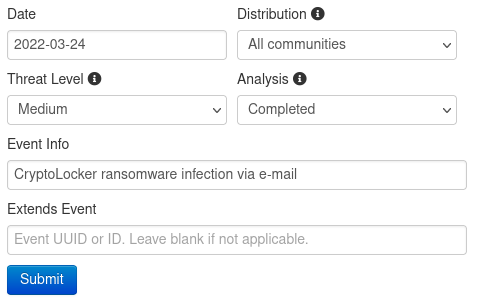
\includegraphics[width=1.0\linewidth]{pictures/case2/event.png}
\end{frame}

\begin{frame}
    \frametitle{Case study 2: Ransomware}
    \begin{itemize}
        \item Add the original e-mail
        \item As the email contains multiple contextually linked data points, we should use an \texttt{Email} \textit{object}
        \item Add contextual comment such as:
        \begin{itemize}
            \item \texttt{Email received by the victim containing the ransomware}
        \end{itemize}
        \item Include at least: \texttt{from}, \texttt{subject} and \texttt{body}
    \end{itemize}
\end{frame}

\begin{frame}
    \frametitle{Case study 2: Ransomware}
    \begin{center}
        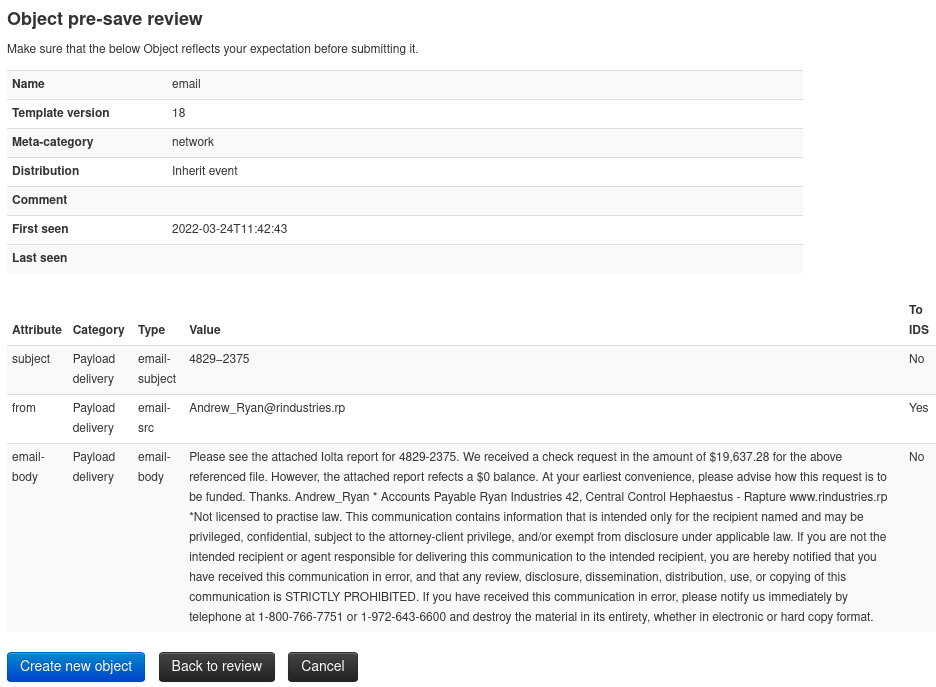
\includegraphics[width=0.9\linewidth]{pictures/case2/object-mail.png}
    \end{center}
\end{frame}

\begin{frame}
    \frametitle{Case study 2: Ransomware}
    \begin{itemize}
        \item Add the ransomware binary as attachment
        \item Pick the \texttt{Payload Delivery} category
        \item Add contextual comment such as:
        \begin{itemize}
            \item \texttt{CryptoLocker ransomware delivered by email}
        \end{itemize}
        \item Check \textit{Is a malware sample}
    \end{itemize}
    \begin{center}
        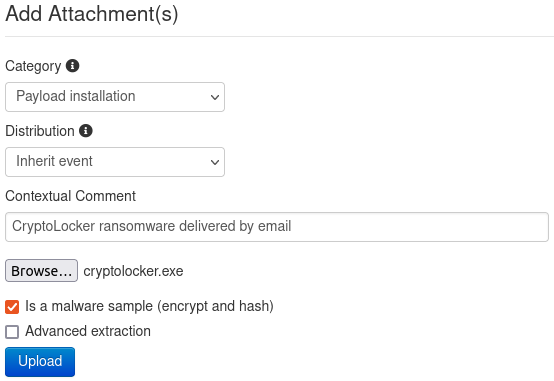
\includegraphics[width=0.70\linewidth]{pictures/case2/attribute-bin.png}
    \end{center}
\end{frame}

\begin{frame}
    \frametitle{Case study 2: Ransomware}
    \begin{itemize}
        \item Encode the IP address of the C2 server with an \textit{attribute}
        \item Pick the \texttt{Payload Installation} category and \texttt{ip-src}  \texttt{type}
        \item Check the \texttt{For Intrusion Detection System}
        \item Add a contextual comment such as
        \begin{itemize}
            \item \texttt{IP address of the scammer collected from the RDP log file}
        \end{itemize}
    \end{itemize}
    \begin{center}
        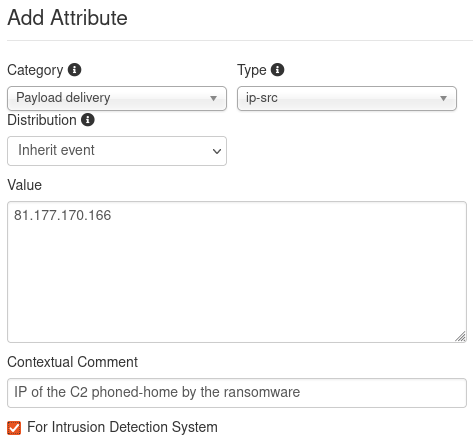
\includegraphics[width=0.42\linewidth]{pictures/case2/attribute-ip.png}
    \end{center}
\end{frame}

\begin{frame}
    \frametitle{Case study 2: Ransomware}
    \begin{itemize}
        \item Encode the registry keys used for persistence by the ransomware
        \item As the registry keys contains multiple contextually linked data points, we should use an \texttt{registry-key} \textit{object}
        \item Add a contextual comment such as
        \begin{itemize}
            \item \texttt{The registry key used for persistence, making sure it gets run again after an OS reboot}
        \end{itemize}
    \end{itemize}
    \begin{center}
        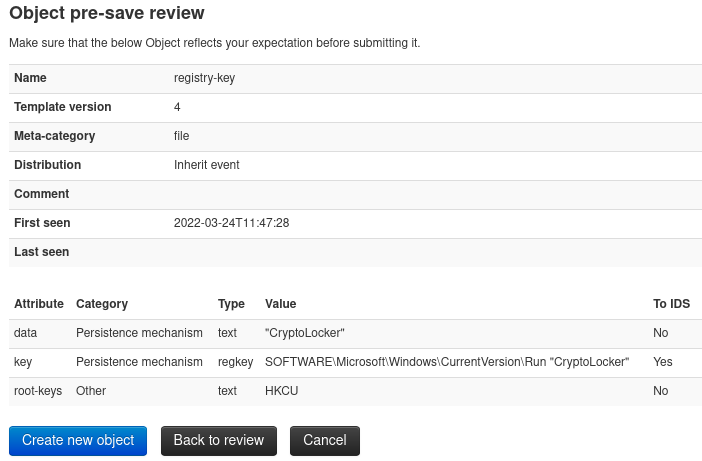
\includegraphics[width=0.61\linewidth]{pictures/case2/object-registry-persistence.png}
    \end{center}
\end{frame}

\begin{frame}
    \frametitle{Case study 2: Ransomware}
    \begin{itemize}
        \item Encode the registry keys used for storing the ransomware's configuration
        \item As the registry keys contains multiple contextually linked data points, we should use an \texttt{registry-key} \textit{object}
        \item Add a contextual comment such as
        \begin{itemize}
            \item \texttt{Containing configuration data (C2 address, malware version and installation timestamp)}
        \end{itemize}
    \end{itemize}
    \begin{center}
        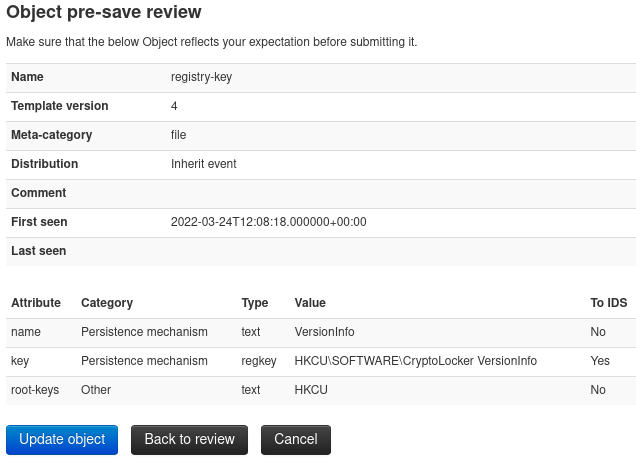
\includegraphics[width=0.55\linewidth]{pictures/case2/object-registry-config.png}
    \end{center}
\end{frame}

\begin{frame}
    \frametitle{Case study 2: Ransomware}
    \begin{itemize}
        \item Encode the registry keys used for ransomware PK
        \item As the registry keys contains multiple contextually linked data points, we should use an \texttt{registry-key} \textit{object}
        \item Add a contextual comment such as
        \begin{itemize}
            \item \texttt{Contains the RSA public key received from the C2 used for encryption}
        \end{itemize}
    \end{itemize}
    \begin{center}
        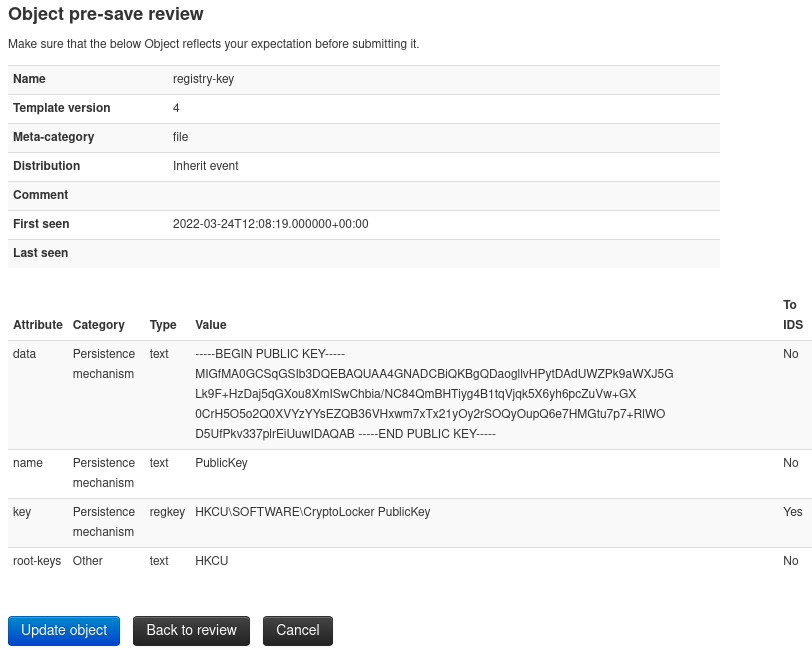
\includegraphics[width=0.55\linewidth]{pictures/case2/object-registry-pb.png}
    \end{center}
\end{frame}

\begin{frame}
    \frametitle{Case study 2: Ransomware}
    \begin{itemize}
        \item Encode the bitcoin address used to reveive the ransom
        \item Pick the \texttt{Financial Fraud} category and \texttt{btc}  \texttt{type}
        \item Check the \texttt{For Intrusion Detection System}
        \item Add a contextual comment such as
        \begin{itemize}
            \item \texttt{Hardcoded address on which the ransom is asked to be transfered}
        \end{itemize}
    \end{itemize}
    \begin{center}
        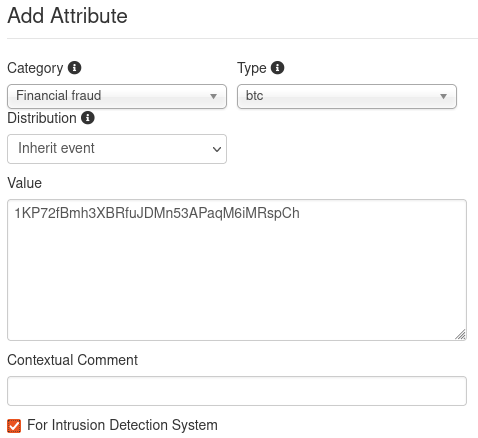
\includegraphics[width=0.47\linewidth]{pictures/case2/attribute-btc.png}
    \end{center}
\end{frame}

\begin{frame}
    \frametitle{Case study 2: Ransomware}
    \begin{itemize}
        \item Encode the name and roles of the person
        \item As these attributes are contextually linked between each others, we should use a \texttt{person} \textit{object}
        \item Add a contextual comment such as
        \begin{itemize}
            \item \texttt{Person from which the mail seems to originate}
        \end{itemize}
        \item Include at least: \texttt{full-name}, \texttt{e-mail} and \texttt{roles}
    \end{itemize}
    \begin{center}
        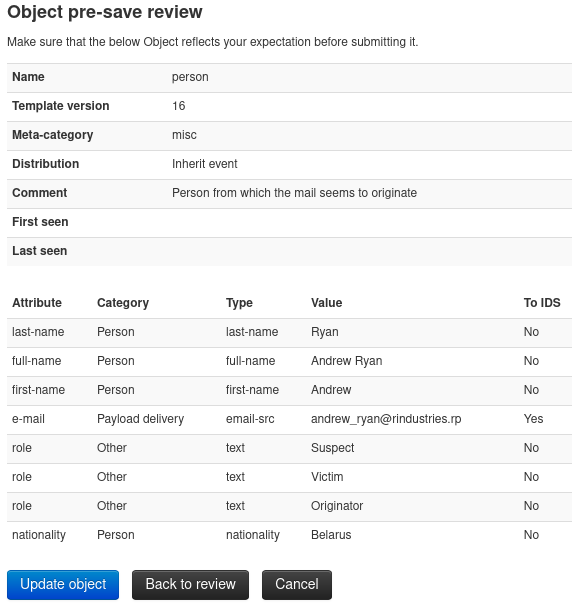
\includegraphics[width=0.42\linewidth]{pictures/case2/object-person.png}
    \end{center}
\end{frame}

\begin{frame}
    \frametitle{Case study 2: Ransomware}
    \begin{itemize}
        % \item Encode the XOR key
        % \item Pick the \texttt{Artifacts dropeed} category and \texttt{hex} \texttt{type}
        % \item Check the \texttt{For Intrusion Detection System}
        % \item Add a contextual comment such as
        % TODO
        \item use crypto material
        \begin{itemize}
            \item \texttt{XOR key used to encode the malware's configuration in the registry}
        \end{itemize}
    \end{itemize}
    \begin{center}
        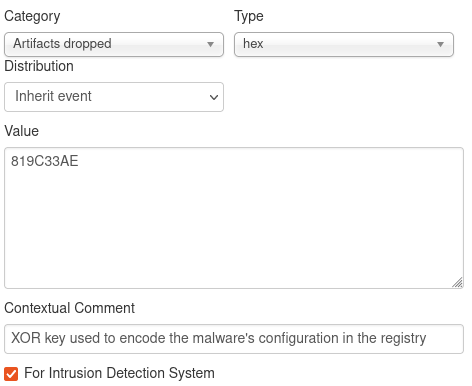
\includegraphics[width=0.47\linewidth]{pictures/case2/attribute-key.png}
    \end{center}
\end{frame}

\begin{frame}
    \frametitle{Case study 2: Ransomware}
    Add (at least) these relationships to recreate the story

    \begin{center}
        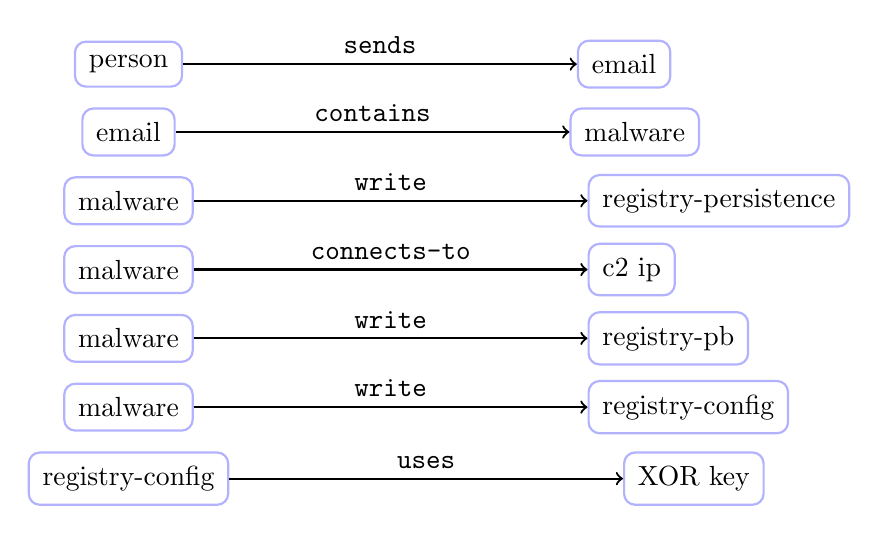
\begin{tikzpicture}[
            entity/.style={rectangle, draw=black, scale=0.7},
            simplebox/.style={
                rectangle, rounded corners, thick,
                draw=blue!30,
                minimum width=10pt,
                minimum height=10pt,
                inner sep=5pt, inner ysep=5pt
            },
        ]

            \node [simplebox] (person1)                     {person};
            \node [simplebox] (mail1) [ right= 5cm of person1 ] {email};
            \draw[->,thick] (person1) -- (mail1) node [above,midway] {\texttt{sends}};

            \node [simplebox] (mail2) [ below= 0.25cm of person1]       {email};
            \node [simplebox] (file1) [ right= 5cm of mail2 ] {malware};
            \draw[->,thick] (mail2) -- (file1) node [above,midway] {\texttt{contains}};

            \node [simplebox] (file2) [ below= 0.25cm of mail2 ] {malware};
            \node [simplebox] (registry-persistence)    [ right= 5cm of file2 ] {registry-persistence};
            \draw[->,thick] (file2) -- (registry-persistence) node [above,midway] {\texttt{write}};

            \node [simplebox] (file5) [ below= 0.25cm of file2 ] {malware};
            \node [simplebox] (ip)    [ right= 5cm of file5 ] {c2 ip};
            \draw[->,thick] (file5) -- (ip) node [above,midway] {\texttt{connects-to}};

            \node [simplebox] (file3) [ below= 0.25cm of file5 ] {malware};
            \node [simplebox] (registry-pb)    [ right= 5cm of file3 ] {registry-pb};
            \draw[->,thick] (file3) -- (registry-pb) node [above,midway] {\texttt{write}};

            \node [simplebox] (file4) [ below= 0.25cm of file3 ] {malware};
            \node [simplebox] (registry-config)    [ right= 5cm of file4 ] {registry-config};
            \draw[->,thick] (file4) -- (registry-config) node [above,midway] {\texttt{write}};

            \node [simplebox] (registry-config2) [ below= 0.25cm of file4 ] {registry-config};
            \node [simplebox] (xor-key)    [ right= 5cm of registry-config2 ] {XOR key};
            \draw[->,thick] (registry-config2) -- (xor-key) node [above,midway] {\texttt{uses}};

        \end{tikzpicture}
    \end{center}
\end{frame}

\begin{frame}
    \frametitle{Case study 2: Ransomware}
    Add relationships to recreate the story
    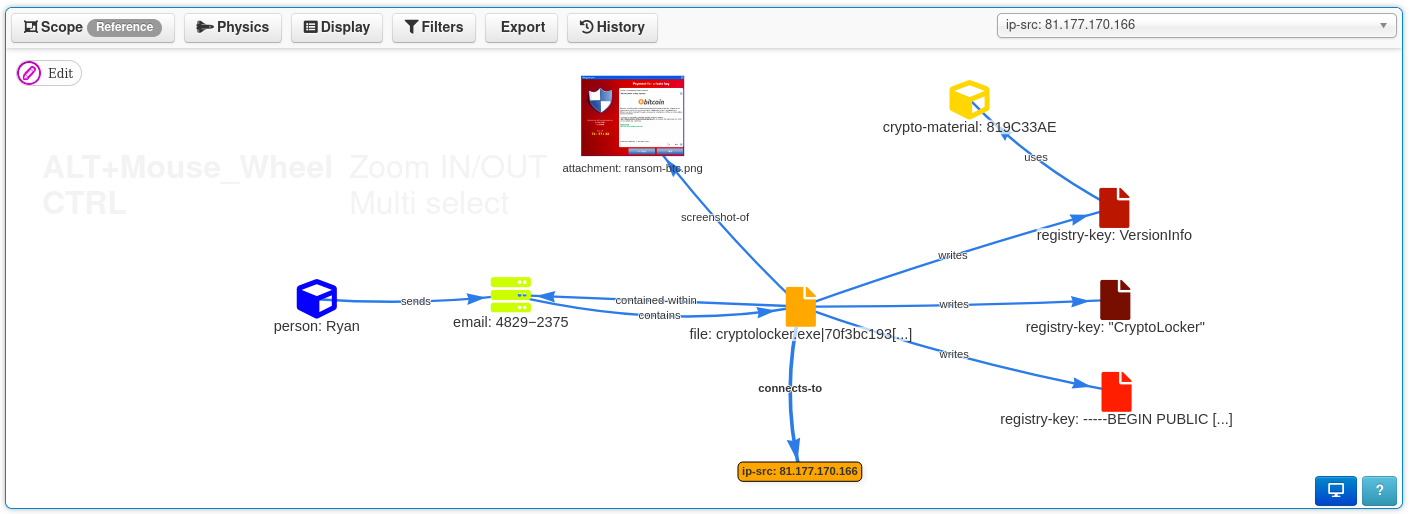
\includegraphics[width=1.0\linewidth]{pictures/case2/event-graph.png}
\end{frame}

\begin{frame}
    \frametitle{Case study 2: Ransomware}
    Add time component to recreate the chronology
    \begin{itemize}
        \item Main focus is the Cyber Threat Intelligence (CTI) aspect
    \end{itemize}
    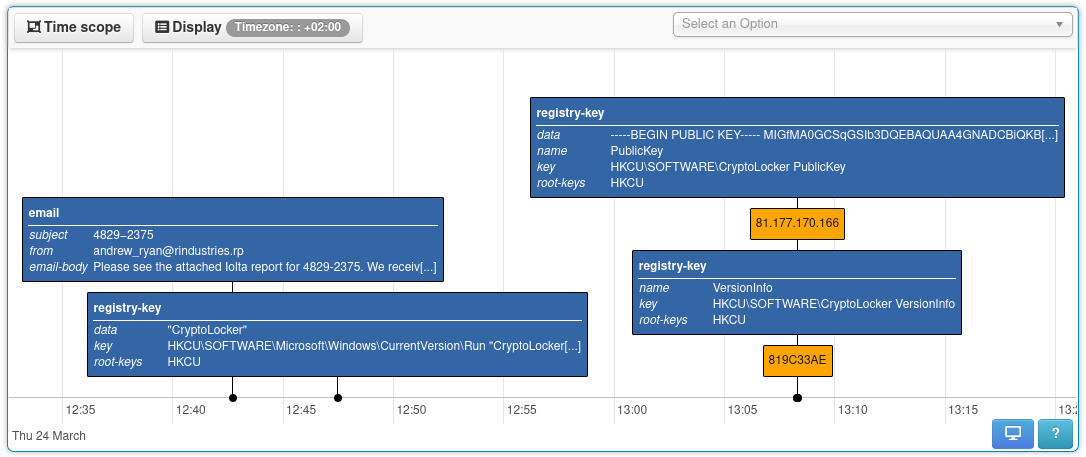
\includegraphics[width=1.0\linewidth]{pictures/case2/timeline.png}
\end{frame}

\begin{frame}
    \frametitle{Case study 2: Ransomware}
    Perform enrichments
    \begin{itemize}
        \item IP address to get its location
    \end{itemize}
    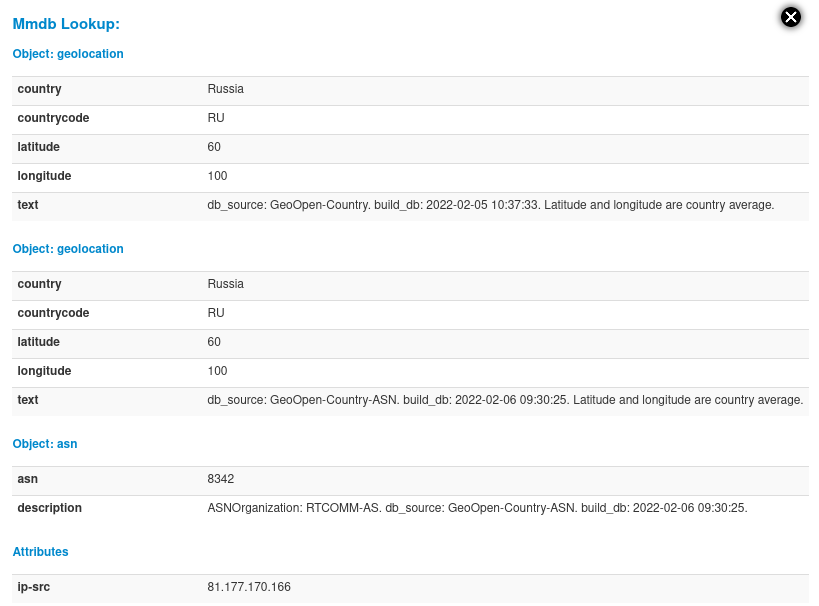
\includegraphics[width=1.0\linewidth]{pictures/case2/enrichment1.png}
\end{frame}

\begin{frame}
    \frametitle{Case study 2: Ransomware}
    Perform enrichments
    \begin{itemize}
        \item Bitcoin wallet to view the transactions
    \end{itemize}
    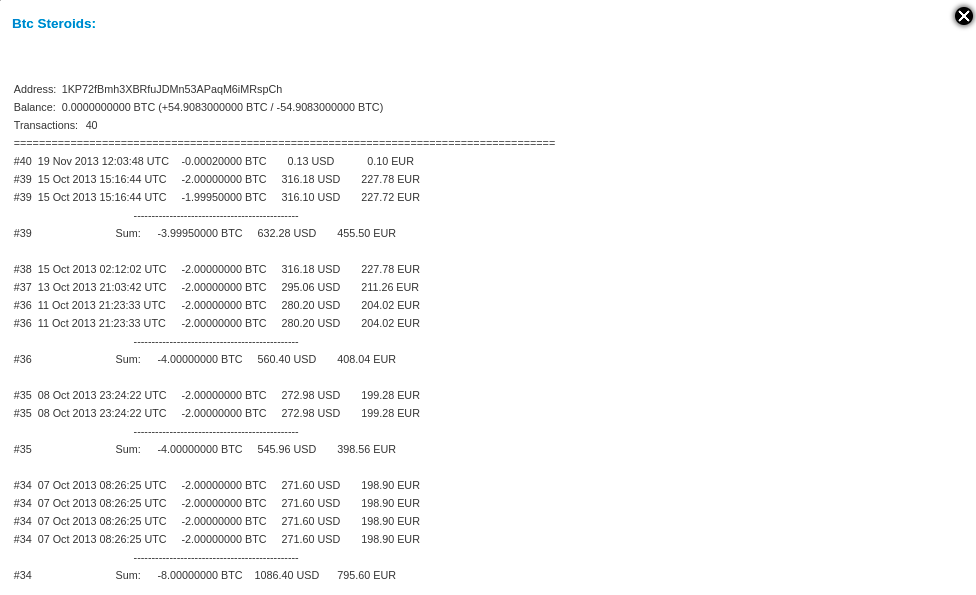
\includegraphics[width=1.0\linewidth]{pictures/case2/enrichment-btc.png}
\end{frame}

\begin{frame}
    \frametitle{Case study 2: Ransomware}
    \begin{itemize}
        \item Contextualizing the data
        \begin{itemize}
            \item Different country / sectors might use different nomemclature
        \end{itemize}
        \item Suggestions of taxonomies for tagging:
        \begin{itemize}
            \item \texttt{adversary}: adversary infrastructure
            \item \texttt{circl}: Classification in Incident Response
            \item \texttt{enisa}: ENISA structuring aid for information and threats
            \item \texttt{europol-*}: Describe the type of events or incidents
            \item \texttt{maec-*}: Malware Attribute Enumeration and Characterization
            \item \texttt{malware\_classification}: Based on SANS malware 101
            \item \texttt{ms-caro-malware}: Microsoft’s Malware Type and Platform
            \item \texttt{ransomware}: ransomware types and the elements
            \item \texttt{veris}: Vocabulary for Event Recording and Incident Sharing 
            \item \texttt{collaborative-intelligence}: Support analysts
            \item \texttt{workflow}: Support analysts
            \item \texttt{tlp}: Traffic Light Protocol 
        \end{itemize}
    \end{itemize}
\end{frame}

\begin{frame}
    \frametitle{Case study 2: Ransomware}
    \begin{itemize}
        \item Incident type
        \begin{itemize}
            \item \texttt{circl:incident-classification="ransomware"}
            \item \texttt{enisa:nefarious-activity-abuse="ransomware"}
            \item \texttt{europol-incident:malware="infection"}
            \item \texttt{europol-incident:malware="c\&c"}
            \item \texttt{ms-caro-malware:malware-type="Ransom"}
        \end{itemize}
        \item Malware type
        \begin{itemize}
            \item \texttt{\scriptsize malware\_classification:malware-category="Ransomware"}
            \item \texttt{ransomware:type="crypto-ransomware"}
        \end{itemize}
        \item Collaration and Sharing
        \begin{itemize}
            \item \texttt{\tiny collaborative-intelligence:request="extracted-malware-config"}
            \item \texttt{workflow:state="complete"}
            \item \texttt{tlp:green}
        \end{itemize}
    \end{itemize}
\end{frame}

\begin{frame}
    \frametitle{Case study 2: Ransomware}
    \begin{itemize}
        \item Infection vector
        \begin{itemize}
            \item \texttt{europol-event:dissemination-malware-email}
            \item \texttt{\tiny maec-delivery-vectors:maec-delivery-vector="email-attachment"}
            \item \texttt{ransomware:infection="phishing-e=mails"}
        \end{itemize}
        \item Adversary infrastructure
        \begin{itemize}
            \item \texttt{adversary:infrastructure-type="c2"}
            \item \texttt{veris:action:malware:variety="C2"}
        \end{itemize}
    \end{itemize}
\end{frame}

\begin{frame}
    \frametitle{Case study 2: Ransomware}
    Malware-specific information
    \begin{itemize}
        \item \texttt{\scriptsize maec-malware-capabilities:maec-malware-capability="fraud"}
        \item \texttt{\tiny maec-malware-capabilities:maec-malware-capability="persistence"}
        \item \texttt{\tiny maec-malware-capabilities:maec-malware-capability="communicate-with-c2-server"}
        \item \texttt{\tiny maec-malware-capabilities:maec-malware-capability="compromise-data-availability"}
        \item \texttt{\scriptsize ransomware:element="ransomnote"}
        \item \texttt{\scriptsize ransomware:element="dropper"}
        \item \texttt{\tiny ransomware:complexity-level="file-restoration-possible-using-shadow-volume-copies"}
        \item \texttt{\tiny ransomware:complexity-level="file-restoration-possible-using-backups"}
        \item \texttt{\tiny ransomware:complexity-level=\\ "decryption-key-recovered-from-a-C\&C-server-or-network-communications"}
        \item \texttt{\tiny ransomware:complexity-level="encryption-model-is-seemingly-flawless"}
        \item \texttt{\scriptsize ransomware:purpose="deployed-as-ransomware-extortion"}
        \item \texttt{\scriptsize ransomware:target="pc-workstation"}
        \item \texttt{\scriptsize ransomware:communication="dga-based"}
        \item \texttt{\scriptsize ransomware:malicious-action="asymmetric-key-encryption"}
    \end{itemize}
\end{frame}

\begin{frame}
    \frametitle{Case study 2: Ransomware}
    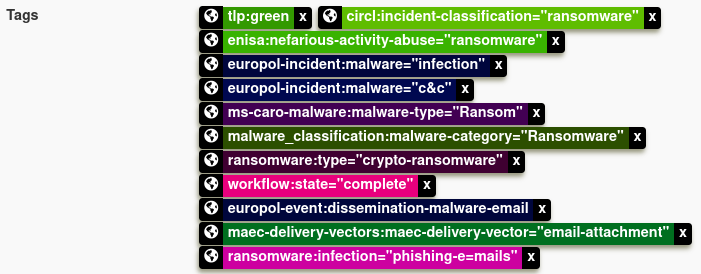
\includegraphics[width=1.0\linewidth]{pictures/case2/event-tags.png}
    \vspace{0.25cm}
    \begin{itemize}
        \item Danger of over-classification
        \begin{itemize}
            \item Make things cluttered and unreadable
            \item Mixing classification scheme
            \item Introduce a non-negligible overhead when using \textit{LIKE} filters (e.g. \texttt{tlp:\%})
        \end{itemize}
    \end{itemize}
\end{frame}

\begin{frame}
    \frametitle{Case study 2: Ransomware}
    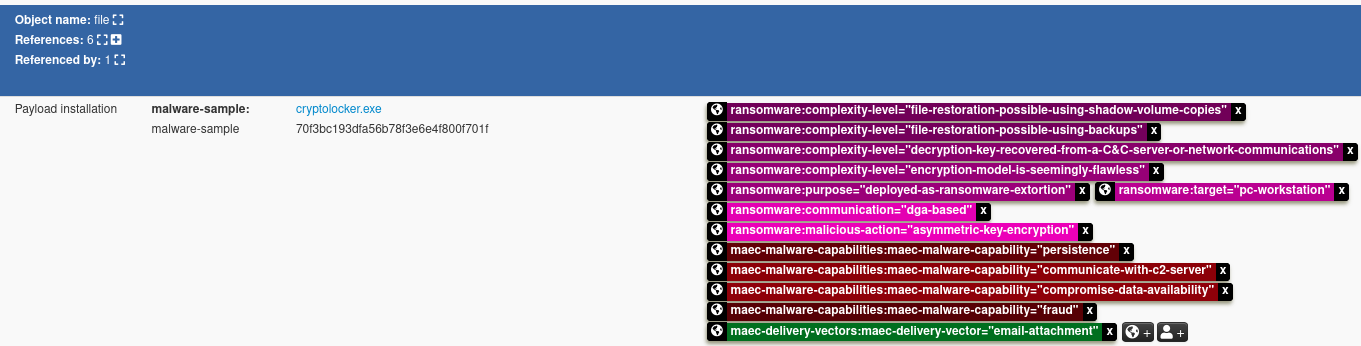
\includegraphics[width=1.0\linewidth]{pictures/case2/attribute-tags1.png}
    \vspace{0.25cm}
    \begin{itemize}
        \item Depending on the community, being complete on the contextualization can be useful for metrics and trends
    \end{itemize}
\end{frame}

\begin{frame}
    \frametitle{Case study 2: Ransomware}
    \begin{itemize}
        \item Adding tags on attribute level make the role of the data clearer
        \item Make searches and exports easier
    \end{itemize}
    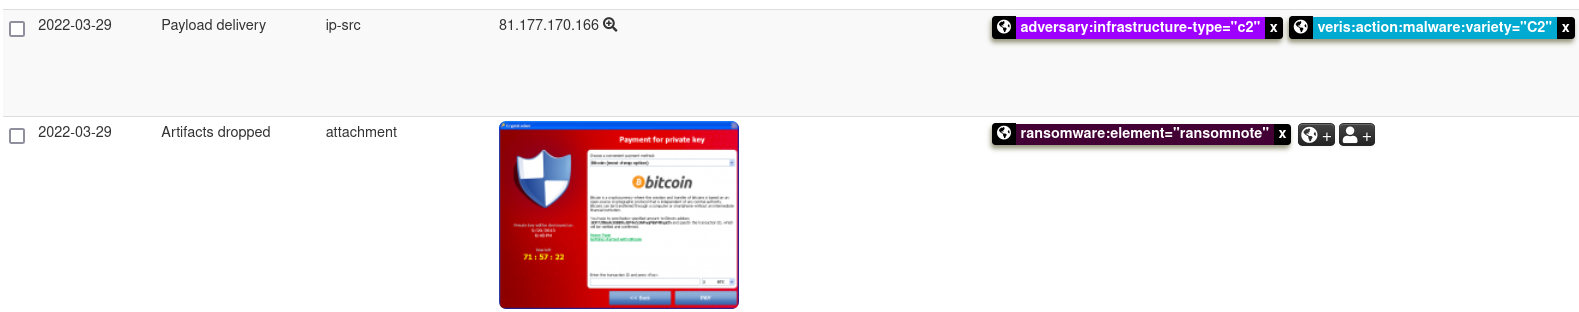
\includegraphics[width=1.0\linewidth]{pictures/case2/attribute-tags2.png}
    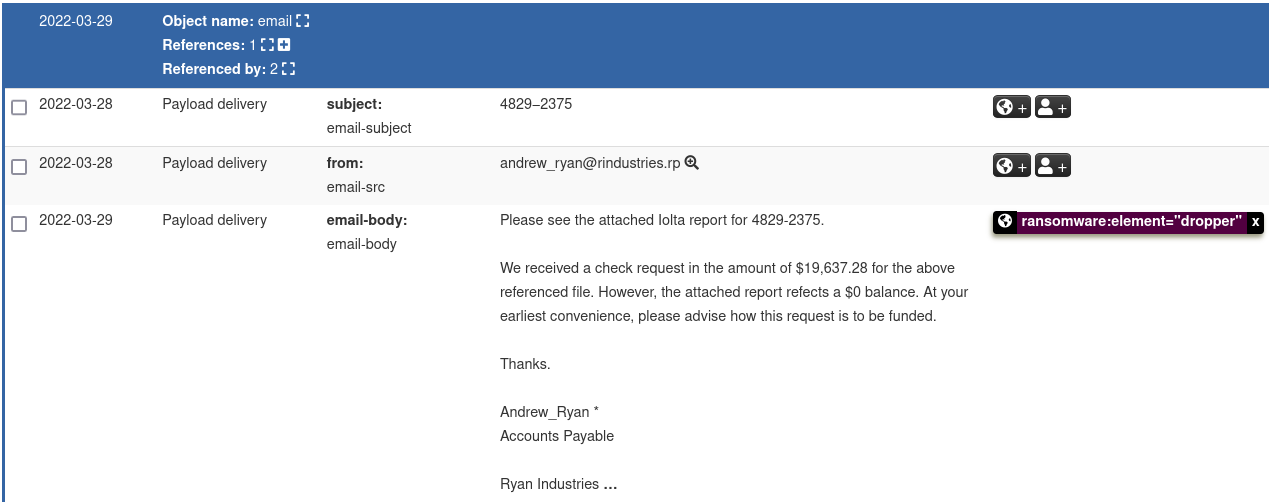
\includegraphics[width=1.0\linewidth]{pictures/case2/attribute-tags3.png}
\end{frame}

\begin{frame}
    \frametitle{Case study 2: Ransomware}
    \begin{itemize}
        \item Contextualizing the data: Galaxy Clusters
        \begin{itemize}
            \item Note: Different country / sectors might use different nomemclature
        \end{itemize}
        \item Suggestions for tagging with Galaxies:
        \begin{itemize}
            \item Malpedia
            \item Ransomware
            \item MITRE Attack Pattern
            \item Preventive Measure
        \end{itemize}
    \end{itemize}
\end{frame}

\begin{frame}
    \frametitle{Case study 2: Ransomware}
    \begin{center}
        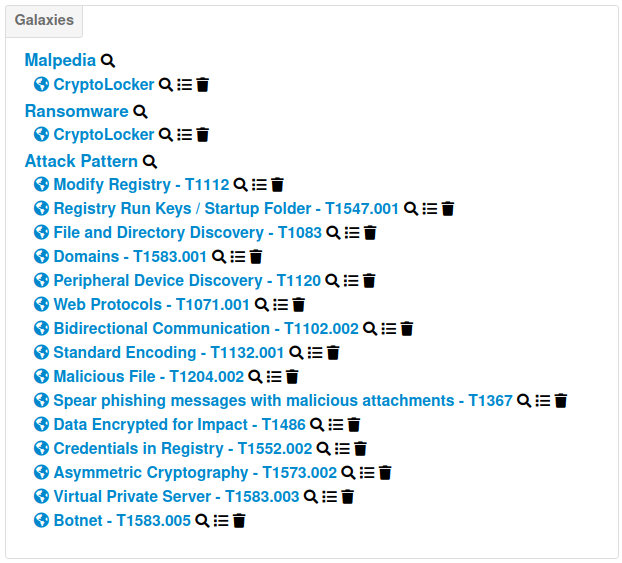
\includegraphics[width=0.80\linewidth]{pictures/case2/event-clusters.png}
    \end{center}
\end{frame}

\begin{frame}
    \frametitle{Case study 2: Ransomware}
    Preventive measures
    \begin{center}
        TODO: Include PM
        % \includegraphics[width=0.80\linewidth]{pictures/case2/event-clusters2.png}
    \end{center}
\end{frame}

\begin{frame}
    \frametitle{Case study 2: Ransomware}
    MITRE ATT\&CK Matrix\\

    \vspace{1cm}
    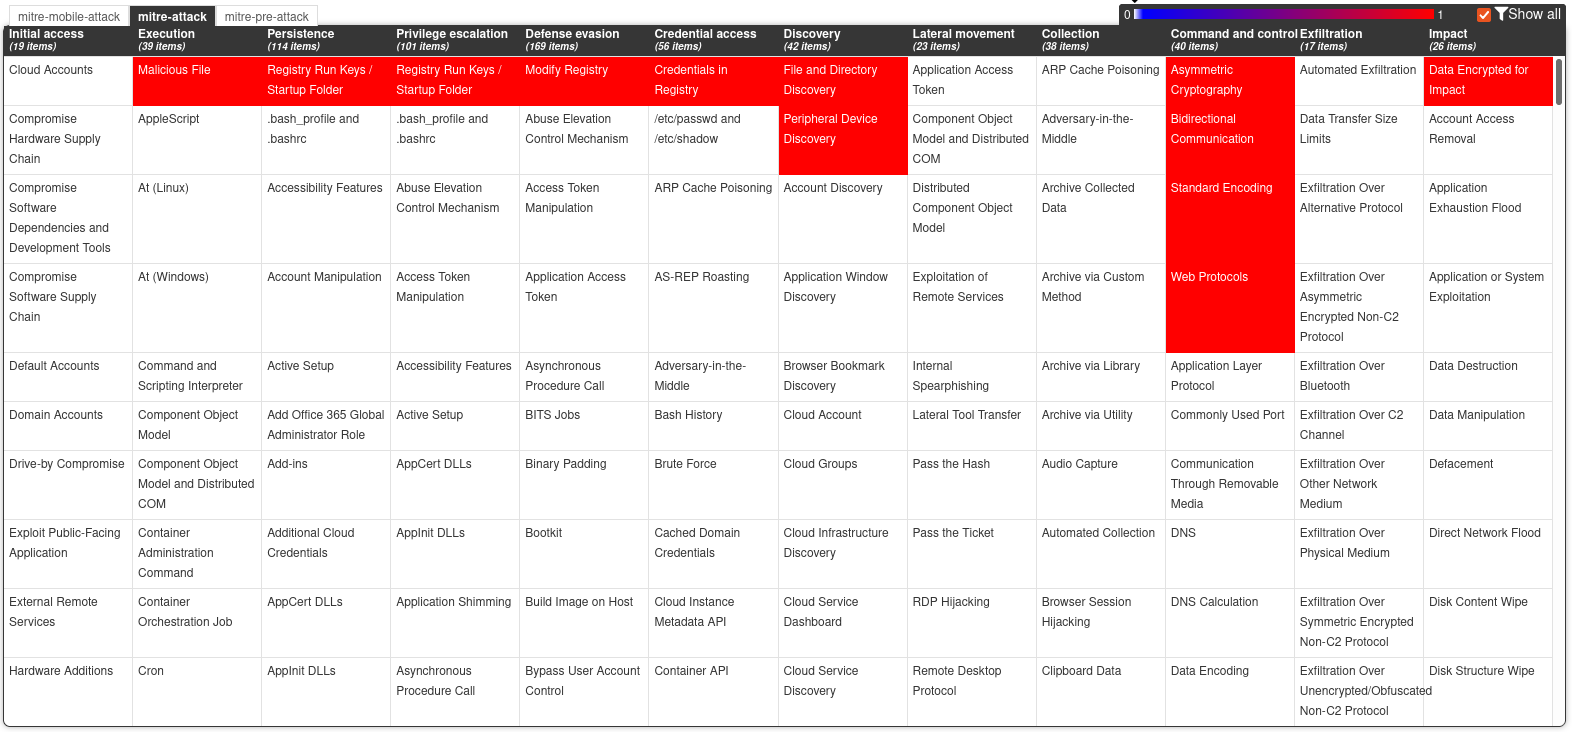
\includegraphics[width=1.0\linewidth]{pictures/case2/event-attack.png}
\end{frame}

\begin{frame}
    \frametitle{Case study 2: Ransomware}
    Create a small write-up as an \textit{event report}
    \begin{itemize}
        \item Create the \textit{event report} with a concise name
        \item Example: Executive summary of the case
        \begin{itemize}
            \item Leave its content empty as it can be edited with more ease in the editor afterward
        \end{itemize}
        \item Write a summary with
        \begin{itemize}
            \item Quick chronology
            \item Written explanation of the steps tooks by the ransomware
            \item Reference to existing \textit{attributes} or \textit{objects} whenever possible
            \begin{itemize}
                \item The special syntax is: \texttt{@[scope]\{uuid\}}
            \end{itemize}
        \end{itemize}
    \end{itemize}
\end{frame}

\begin{frame}
    \frametitle{Case study 2: Ransomware}
    \begin{itemize}
        \item Create a small write-up as an \textit{event report}
        \item We could have a technical report and another one for the incident
    \end{itemize}
    \begin{center}
        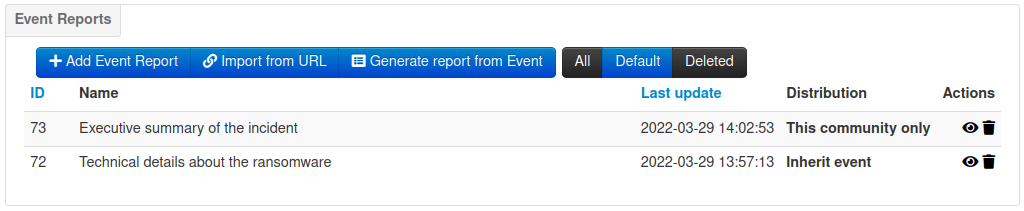
\includegraphics[width=1.0\linewidth]{pictures/case2/event-report-list.png}
    \end{center}
\end{frame}

\begin{frame}
    \frametitle{Case study 2: Ransomware}
    \begin{center}
        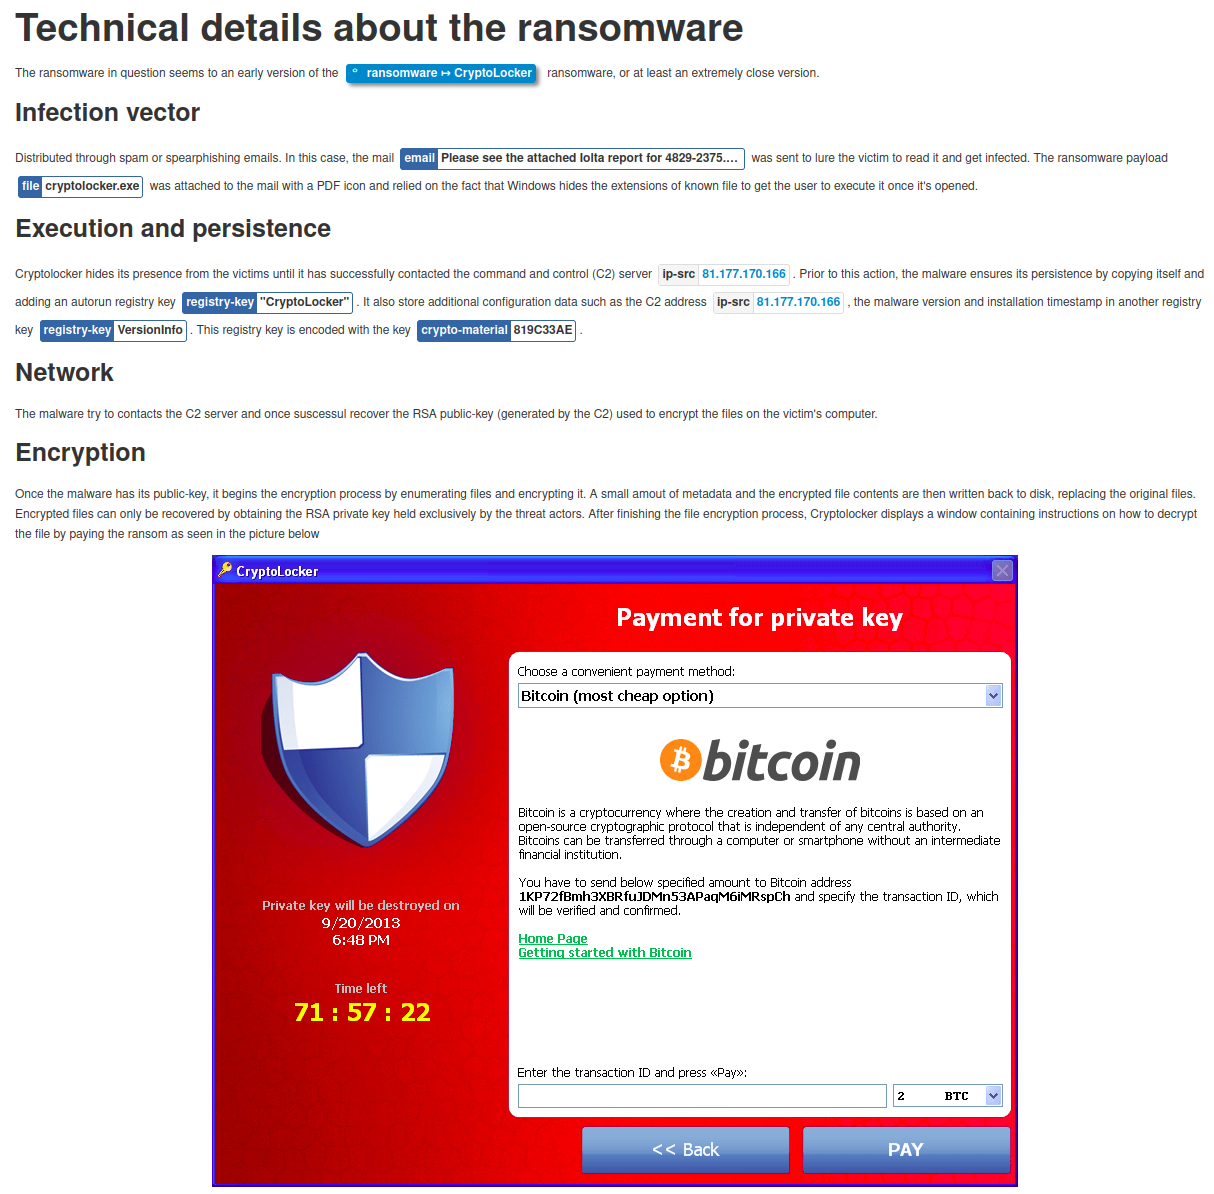
\includegraphics[width=0.65\linewidth]{pictures/case2/event-report-2.png}
    \end{center}
\end{frame}

\begin{frame}
    \frametitle{Case study 2: Ransomware}
    \begin{center}
        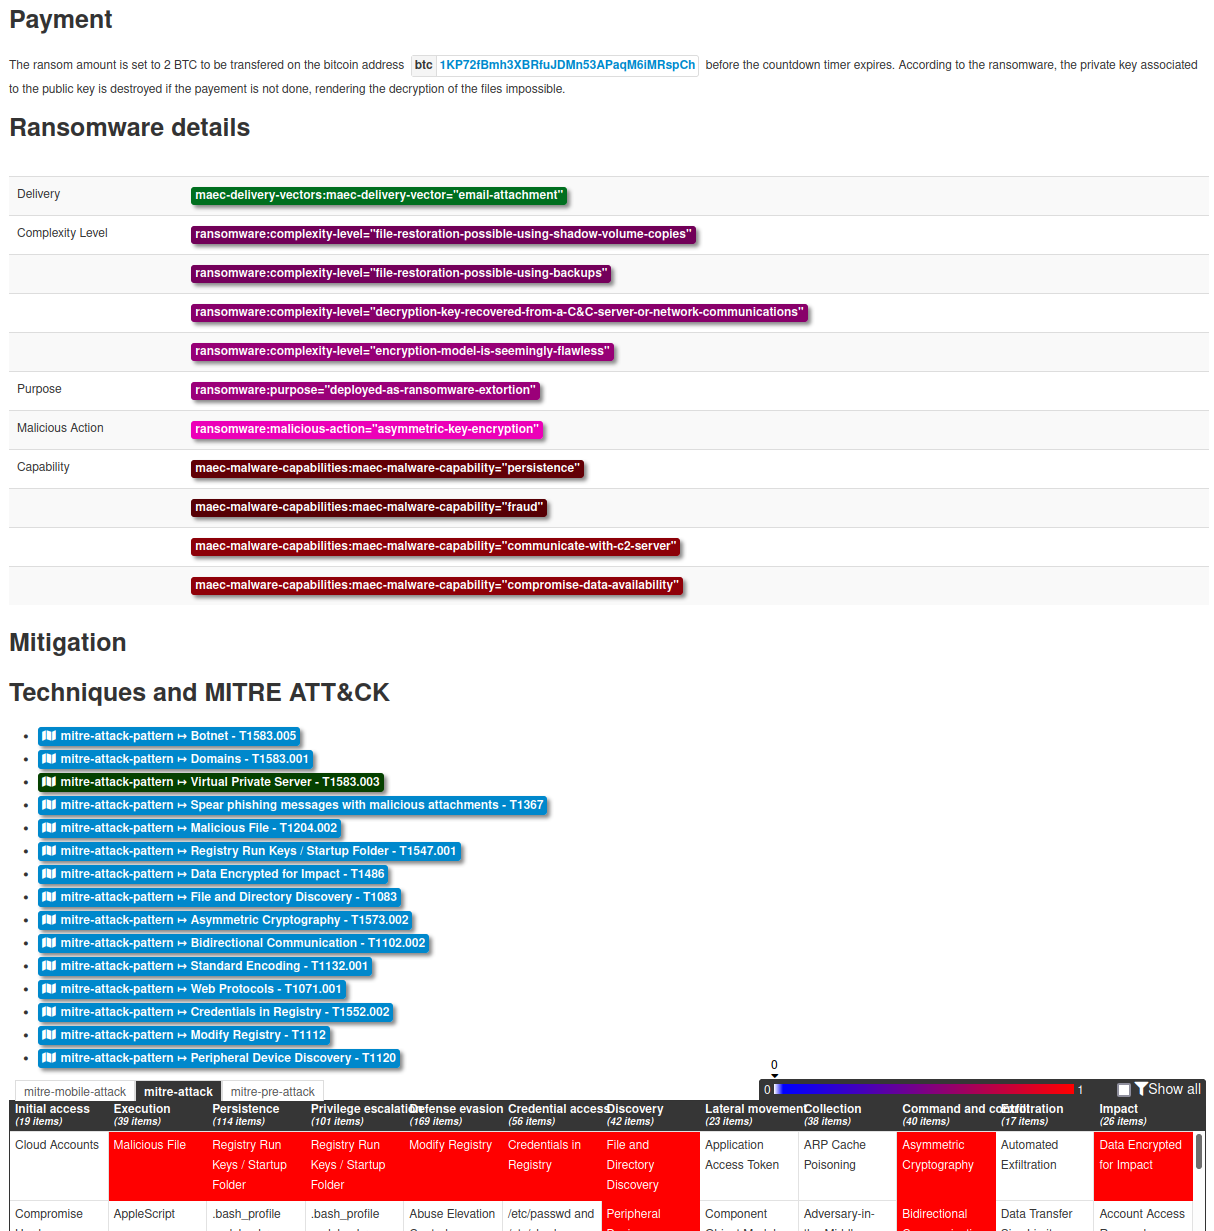
\includegraphics[width=0.65\linewidth]{pictures/case2/event-report-3.png}
    \end{center}
\end{frame}

\begin{frame}
    \frametitles{Case study 2: Ransomware}{Review the distribution level and publish}
    In our case, we consider the following MISP network topology
    \begin{itemize}
        \item The current instance is owned and managed by a LEA
        \item The current instance is connected to a central MISP instance acting as a "Hub"
        \item The "Hub" is connected to various other MISP instances such as other LEAs, CSIRTs, Financial and telecom institutions
    \end{itemize}

    \begin{center}
        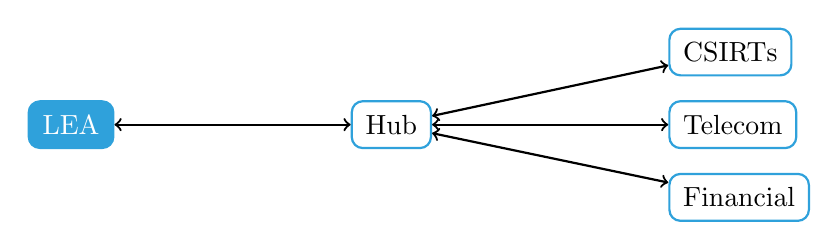
\begin{tikzpicture}[
            entity/.style={rectangle, draw=black, scale=0.7},
            simplebox/.style={
                rectangle, rounded corners, thick,
                draw=main,
                minimum width=10pt,
                minimum height=10pt,
                inner sep=5pt, inner ysep=5pt
            },
        ]
            \node [simplebox] (hub)                     {Hub};
            \node [simplebox,fill=main] (lea) [ left= 3cm of hub ] {\textcolor{white}{LEA}};
            \node [simplebox] (csirts) [ above right = 0.3cm and 3cm of hub ] {CSIRTs};
            \node [simplebox] (telecom) [ right= 3cm of hub ] {Telecom};
            \node [simplebox] (financial) [ below right= 0.3cm and 3cm of hub ] {Financial};

            \draw[<->,thick] (lea) -- (hub) node [above,midway] {};
            \draw[<->,thick] (csirts) -- (hub) node [above,midway] {};
            \draw[<->,thick] (telecom) -- (hub) node [above,midway] {};
            \draw[<->,thick] (financial) -- (hub) node [above,midway] {};

        \end{tikzpicture}
    \end{center}
\end{frame}

\begin{frame}
    \frametitle{Case study 2: Ransomware}
    Review the distribution level and publish
    \begin{itemize}
        \item \texttt{binary file}: \textbf{All communities}
        \item \texttt{C2 ip} \& \texttt{geolocation}: \textbf{All communities}
        \item \texttt{crypto-material} \& \texttt{registry-keys}: \textbf{All communities}
        \item \texttt{person}: \textbf{All communities}
        \begin{itemize}
            \item Even though \texttt{Andrew Ryan} could be a victim due to impersonation, it's very likely that's a fake name
            \item The email address \texttt{andrew\_ryan@rindustries.rp} IoC outweights the risk
        \end{itemize}
    \end{itemize}
    \begin{center}
        \textbf{$\rightarrow$ Publish the event!}
    \end{center}
\end{frame}

\end{document}

